\documentclass[12pt]{article}

%\usepackage[utf8]{inputenc}
%\usepackage[english]{babel}

%
% COLORS
%
\usepackage[dvipsnames, table]{xcolor}{\rm }

%
% LINKS AND REFERENCES
%
\usepackage{hyperref}
\hypersetup{
	colorlinks,
	linkcolor={Red!90!black},
	citecolor={Red!90!black},
	urlcolor={Red}
}

\usepackage{geometry}

\usepackage[parfill]{parskip} % https://tex.stackexchange.com/a/16703/135296

% sub figures / grids of pictures
\usepackage{subcaption}
\usepackage{graphicx}
\graphicspath{{img/}} % includegraphics path
\newcommand{\includegraphicsw}[2][1.]{\includegraphics[width=#1\linewidth]{#2}}
\newcommand{\svginput}[1]{\input{img/#1}} % pdf_tex path
\newcommand{\svginputw}[2][\linewidth]{\def\svgwidth{#1}\input{img/#2}} % pdf_tex path
% pdf
\usepackage{pdfpages}
% tables
\usepackage{multirow}
\usepackage{hhline}
\usepackage{colortbl}
\usepackage{wrapfig}
% \coloneqq
\usepackage{mathtools}
\usepackage{amssymb}
\usepackage{amsthm} % proofs
\usepackage{stmaryrd} % llbracket for jumps
% bold for everything
\usepackage{bm}
%\usepackage{showlabels}
% lowercase mathcal font
\usepackage{dutchcal}

% braces for subeqns and boxes
\usepackage{empheq}
% http://mirror.hmc.edu/ctan/macros/latex/contrib/mathtools/empheq.pdf
\newcommand*\widefbox[1]{\fbox{\hspace{1em}#1\hspace{1em}}}

% math commands for convinience
\DeclareMathOperator{\argmin}{arg\,min}
\DeclareMathOperator{\Span}{span}
% bold vectors
\newcommand{\vect}[1]{\boldsymbol{\mathbf{#1}}}

\newcommand{\bcell}{T}
\newcommand{\bmesh}{{\vect{\mathcal T}}}
\newcommand{\mcell}{\tau}
\newcommand{\mmesh}{{\vect{\mathcal \tau}}}
\newcommand{\bface}{F}
\newcommand{\bfaces}[1][]{{\vect{\mathcal F}_{\text{#1}}}}
\newcommand{\mface}{f}
\newcommand{\mfaces}[1][]{{\vect{\mathcal f}_{\text{#1}}}}

\newcommand{\LTwo}{{\mathbb L^2}}
\newcommand{\lTwo}{{\ell^2}}
\newcommand{\HDiv}{{\mathbb H_\text{div}}}
\newcommand{\Rn}[1]{{\mathbb R^{#1}}}
\newcommand{\Pn}[1]{{\mathbb P^{#1}}}
\newcommand{\LTwoSpace}[1][\Omega]{{\mathbb L^2\left({#1}\right)}}
\newcommand{\lTwoSpace}[1][\Omega]{{\ell^2\left({#1}\right)}}
\newcommand{\HDivSpace}[1][\Omega]{{\mathbb H_\text{div}\left({#1}\right)}}
\newcommand{\HDivNodeSpace}[1][\Omega]{{\mathbb H_\text{div,\,0}\left({#1}\right)}}
\newcommand{\HHalfSpace}[1][\bface]{{\mathbb H^{\frac{1}{2}}\left({#1}\right)}}
\newcommand{\PnSpace}[2]{{\mathbb P^{#1}\left({#2}\right)}}
\newcommand{\HSpace}[1]{{\mathbb H^{#1}\left(\Omega\right)}}

\newcommand{\errlTwo}[1]{e^{\lTwo}_{#1}}
\newcommand{\errInf}[1]{e^{\infty}_{#1}}
\newcommand{\MO}[1]{{\color{blue}MO: #1}}
\newcommand{\DS}[1]{{\color{blue}DS: #1}}
\newcommand{\Sasha}[1]{\colorbox{Cyan}{\textbf{Sasha}:} #1}
\newcommand{\toDiscuss}[1]{\colorbox{Cyan}{\textbf{\,!\,}:} #1}

% differentials
\newcommand*\diff{\mathop{}\!\mathrm{d}}
\newcommand*\Diff[1]{\mathop{}\!\mathrm{d^#1}}

\DeclareMathOperator{\Ker}{ker}
\DeclareMathOperator{\Dim}{dim}

\newtheorem{theorem}{Theorem}[section]
\newtheorem{corollary}{Corollary}[theorem]
\newtheorem{lemma}[theorem]{Lemma}

\newgeometry{
	left=3cm, right=2.5cm, top=1.5cm, bottom=1.5cm,
	includefoot, heightrounded
}

\title{A higher order approximate static condensation method for multi-material diffusion problems}
\author{
	Alexander Zhiliakov\thanks{Department of Mathematics, University of Houston, Houston, Texas 77204 (alex@math.uh.edu).}
	\and Daniil Svyatskiy\thanks{Los Alamos National Laboratory, Los Alamos,
		New Mexico, USA (dasvyat@lanl.gov).}
	\and
	Maxim Olshanskii\thanks{Department of Mathematics, University of Houston, Houston, Texas 77204 (molshan@math.uh.edu); Partially supported by NSF through grant  DMS-1717516.}
	\and Evgeny Kikinzon \thanks{Los Alamos National Laboratory, Los Alamos,
		New Mexico, USA (kikinzon@lanl.gov).}
	\and Mikhail Shashkov\thanks{Los Alamos National Laboratory, Los Alamos,
		New Mexico, USA (shashkov@lanl.gov).}
}

\begin{document}
	
	\maketitle
	
	\let\oldtabular\tabular
	\renewcommand{\tabular}[1][1.5]{\def\arraystretch{#1}\oldtabular}
	
	%\let\oldarray\array
	%\renewcommand{\array}[1][2pt]{\arraycolsep=#1\def\arraystretch{1.5}\oldarray}
	
	\begin{abstract}
		The paper studies an approximate static condensation method for the diffusion problem with discontinuous diffusion coefficients. The method allows for a general polygonal mesh which is unfitted to the material interfaces. Moreover, the interfaces can be discontinuous across the mesh edges as typical for numerical reconstructions using the volume or moment-of-fluid methods.  We apply a mimetic finite difference method to solve local diffusion problems and use $P_1$ (mortar) edge elements to couple local problems into the global system. The condensation process and the properties of the resulting algebraic system are discussed. It is demonstrated that the method is second order accurate on smooth solutions and performs well for problems with high contrast in diffusion coefficients. Experiments also show the robustness with respect to position of the material interfaces against the underlying mesh.
	\end{abstract}
	
	%\Sasha{Note that \texttt{usepackage\{dutchcal\}} seems to be not working with miktex (I need this package for a bold mathcal font). I use texlive and it works just ok. I left it commented so it compiles more or less everywhere. You may see some funny symbols from time to time  while reading if you leave it commented.}
	
	\section{Introduction}
	
	Multi-phase and multi-material processes are ubiquitous in nature and engineering.
	Mathematical models of such processes are often formulated in terms of systems of partial differential equations with discontinuous coefficients and interface conditions on time-dependent internal boundaries.
	Due to their high complexity, these models defy analytical treatment, and hence numerical simulations became an indispensable tool for solving the models and gaining insights into underlying phenomena.
	
	Past decades evidenced an explosive growth in developing of efficient computational techniques for problems with evolving interfaces, which involve interaction between many materials or different phases of matter. These developments include immersed boundary method~\cite{peskin2002immersed}, immersed interface method~\cite{leveque1994immersed}, and unfitted finite element methods \cite{belytschko2009review,burman2015cutfem}, to name several popular numerical approaches. Depending on how the interface is treated numerically, one can distinguish between methods that smear the interface over a strip of finite thickness which should be further resolved by the mesh, like in the phase field approach~\cite{steinbach2009phase}, and methods that use a sharp interface representation, as in the level-set method \cite{sethian1999level}.  If one applies a sharp representation to handle complex geometries or interfaces undergoing large deformations, it is convenient to allow the  interface to cut through the background mesh in an arbitrary way. In turn, this leads to the problem of building accurate and stable approximations for  so-called multi-material cells, i.e. the mesh cells intersected by material interfaces. In particular, one is interested in discretizations which are robust with respect to how interfaces intersect the mesh and with respect to the contrast of  material properties, e.g. the ratio of physical parameters. This is the setting and the problem  we focus in this paper.

%However, numerous applications require local conservation of material volumes on computational meshes that do not explicitly track material interfaces. This is typical for simulations of high speed multi-material flows, where shocks and vorticity often require the use of the Arbitrary Lagrangian-Eulerian method. The complication with this method is that over the course of simulation, material interfaces become unaligned with the computational mesh, with their shape and position inside mesh cells not being explicitly known.
	
One standard approach to handle  multi-material cells is a homogenization procedure. In this approach, one assigns to the cells  artificial homogeneous  material properties, which are calculated based on the volumetric shares of different materials in each of the multi-material cells. This enables one to apply standard discretization thechniques. %if one needs to solve for other physics, such as the heat transfer, on every time step of the simulation.
     %Then, ad-hoc methods can be used to interpolate the solution for the contained materials based on
Further one recovers solution in each phase from the computed cell-averaged values~\cite{dawes2013solving}.
Although being technologically straightforward, the homogenization approach often fails  to accurately model subcell material interactions, which results in non-physical numerical solutions to problems with high-contrast material properties.

As an alternative to the homogenization, one may reconstruct interfaces in each  multi-material cell  using a piecewise planar approximation. In this case, single-material domains  in the cell are  non-overlapping polytopes that typically preserve known material volumes.
%The alternatives generally require for the so-called interface reconstruction to be used in order to approximate material interfaces inside multi-material cells. Interface reconstruction methods typically represent materials in a cell by non-overlapping single-material polytopes that match given volume fractions.
%The most popular approach is based on using a single linear interface to represent an interface between two materials, and is commonly called the Piecewise-Linear Interface Calculation (PLIC).
In this paper, we deal with interfaces reconstructed by the volume-of-fluid (VOF)~\cite{hirt1981volume} method, which is a commonly used numerical  approach to recover interface location. The approach includes the moment-of-fluid (MOF) methods~\cite{ahn2009adaptive} that generally provide better accuracy if centroids of material subdomains are known.
For the numerical experiments here we apply the extended MOF~\cite{kikinzon2018xmof}  to construct local meshes inside multi-material cells such that subcell contains only one material and all information about the local topology is available.
% MAxim: It was not clear why you particularly mention  X-MOF. So I assume that it is what you use for experiments.

%A drawback of interface reconstruction is that reconstructed material interfaces are discontinuous on the interfaces between multi-material cells.
The conservation properties of the  VOF and MOF approaches, however, come at a price of recovering a piecewise planar interface approximation that is  discontinuous across the faces of the background computational mesh.
One technique to deal with this issue consists in including the local tessellations into the global computational mesh, thus effectively refining the mesh so that every cell contains only one material~\cite{garimella2011supermesh}. This turns out to be a non-trivial computational geometry problem, and the resulting mesh in 2D often contains very small and co-linear faces, while the extension of this approach to 3D does not seem feasible for general unstructured meshes.

	In this paper, we devise  a higher order method for the numerical solution of the diffusion problem with discontinuous coefficients on polytopal meshes with multi-material cells. We assume that interface reconstruction is performed using the extended MOF method, which provides local single-material meshes with full topological data. One might consider solving this problem with Nitsche’s methods used in the framework of cut-cells~\cite{burman2015cutfem, hansbo2002unfitted} or extended finite element methods (X-FEM)~\cite{dolbow2008xfem}. However, these methods are typically not locally conservative
%, and interface reconstruction is usually used when volume conservation is a requirement. Additionally,
and the discontinuity of material interfaces across faces of multi-material cells can be large enough to result in a significant loss of accuracy.
	
 The present method builds upon the approximate static condensation (ASC) algorithm proposed in~\cite{kikinzon2017approximate}; it admits high-contrast diffusion coefficients and discontinuous reconstruction of the interfaces. The ASC approach uses the formulation of the interface diffusion problem as a system of problems on local meshes that are coupled through the concentration values and fluxes on the faces of multi-material cells. This face concentration serves as a new primal unknown and it is further approximated by piecewise  polynomial functions defined on all faces of the global (unfitted polygonal) mesh. The original paper ~\cite{kikinzon2017approximate} considered $P_0$ (piecewise constant) approximation to the face concentration, while the present study introduces higher order polynomials for this purpose.
	Although the latter potentially leads to more accurate results  (and in some cases we shall see that it provides convergent results, when the $P_0$ version fails), it also raises some questions about stability and robustness, which we address in the present report.
We note that using a skeleton space of  piecewise polynomial functions to couple local unknowns renders the approach as
a version of a mortar method~\cite{yotov2009mortar,mortar}, although mortar finite element  methods were developed for different types of problems and substantially vary in terms of implementation.
	%One might note that using $P_1$ (piecewise linear) approximation to the face concentration puts the proposed method into the framework of mortar methods~\cite{yotov2009mortar,mortar}. While those methods were developed for different types of problems and substantially differ in terms of implementation, the proposed method fits their high-level formulation.
	
%The approximate static condensation approach leaves much freedom in the choice of the discretization method for the local diffusion problems.  Posed in each polygonal cell, these problems are given by diffusion equations with discontinuous coefficients. On the other hand, local meshes produced by extended interface reconstruction methods, unlike the the global mesh, contain only single-material cells. Following~\cite{kikinzon2017approximate}, we apply the mimetic finite difference (MFD) method from~\cite{lipnikov2014mimetic} to approximate the local diffusion problems on these local meshes.

The approximate static condensation approach leaves much freedom in the choice of the discretization method for the local diffusion problems.  Posed in each polygonal cell, these problems are given by  diffusion equations with  discontinuous coefficients. The method benefits from the observation that   for any fixed cell $T$,  material interfaces, which possibly intersect with $T$,  induce a \emph{consistent polygonal subdivision} (local mesh) of $T$. Opposite to the global mesh, the local one is \emph{fitted} to interfaces, i.e. each micro polyhedral element is shared only by one material. Following~\cite{kikinzon2017approximate}, we apply the mimetic finite difference (MFD) method from~\cite{lipnikov2014mimetic} to approximate the local diffusion problems on this fine fitted mesh.
	After eliminating inter-cell degrees of freedom (d.o.f.), one obtains a system of linear algebraic equations for the face concentration degrees of freedom. The fluxes and inter-element degrees of freedom are recovered by simple postprocessing. Further, we study the performance of the method in terms of accuracy, robustness with respect to the interfaces position,  and algebraic stability.
	
	The remainder of the paper is organized as follows. In section~\ref{sec:model} we formulate the model diffusion problem with discontinuous diffusion tensor, introduce the basic mesh and discuss a reformulation of the model as a system of coupled local problems. Section~\ref{sec:ASC} presents the method and discusses certain  properties of the resulting  system of algebraic equations. Finally, section~\ref{sec:num} collects results of numerical experiments. These results include accuracy tests, numerical comparison with the method from  \cite{kikinzon2017approximate} and with a homogenization method as the alternative approach.
	
	\section{Model problem and macro-mesh decomposition} \label{sec:model}
	
	In a polygonal bounded domain $\Omega \subset \Rn{2}$  we consider the following diffusion problem in the mixed form
	\begin{equation}\label{dual}
		\arraycolsep=2pt\def\arraystretch{1.5}
			\left\{\begin{array}{rcrccl}
			\vect K^{-1}\,\vect u & + & \nabla\,p & = & 0 &\quad\text{in } \Omega , \\
			\nabla\cdot\vect u    & + & c\,p      & = & f &\quad\text{in } \Omega
		\end{array}\right.
	\end{equation}
	with boundary data
	\begin{equation}
		p = g_D \quad\text{on } \partial\Omega_D,\qquad %\label{dual:bc:dirichlet} \\
		\vect u \cdot \hat{\vect n} = g_N \quad\text{on } \partial\Omega_N. \label{dual:bc}
	\end{equation}
	Here $p$ is a concentration and $\vect u$ is the diffusive flux, $\vect K$ is the positive definite  symmetric diffusivity tensor, which we assume constant within each material subdomain, $c\ge0$ is the reaction coefficient, $\hat{\vect n}$ is the outward normal vector to $\partial\Omega$, $g_D$ and $g_N$ are Dirichlet and Neumann boundary data, respectively. In the context of fluid flows in porous media, \eqref{dual}--\eqref{dual:bc} is also known as the Darcy problem. In this case, $p$ has the meaning of pressure, $\vect u$ is fluid velocity, and $\vect K$ is the permeability tensor.
	
	\begin{figure}[h]
		\centering
		\begin{subfigure}{.33\linewidth}
			\centering
			\includegraphicsw{ring_base_voronoi.png}
			\caption{Macro-mesh}
			\label{fig:problem_geometry:base_mesh}
		\end{subfigure}%
		\hfill
		\begin{subfigure}{.33\linewidth}
			\centering
			\includegraphicsw{ring_mmcs_voronoi.png}
			\caption{MMCs}
			\label{fig:problem_geometry:mmcs}
		\end{subfigure}%
		\hfill
		\begin{subfigure}{.33\linewidth}
			\centering
			\includegraphicsw{ring_mini_voronoi.png}
			\caption{MOF reconstruction}
			\label{fig:problem_geometry:mof}
		\end{subfigure}
		\begin{subfigure}{.33\linewidth}
			\centering
			\includegraphicsw{ring_base_voronoi_refined.png}
		\end{subfigure}%
		\hfill
		\begin{subfigure}{.33\linewidth}
			\centering
			\includegraphicsw{ring_mmcs_voronoi_refined.png}
		\end{subfigure}%
		\hfill
		\begin{subfigure}{.33\linewidth}
			\centering
			\includegraphicsw{ring_mini_voronoi_refined.png}
		\end{subfigure}
		\caption{The figure illustrates global unstructured polyhedral mesh (left); Physical interfaces for three materials and cut cells, i.e. multi-material cells (central); The piecewise-planar discontinuous reconstruction of the interfaces by the moment-of-fluid method (right). Everything is shown for two refinement level of the macro-mesh \label{fig:problem_geometry}}
	\end{figure}
	
	We assume the triangulation  $\bmesh$ of $\Omega$ consisting of general polyhedral elements as illustrated in Figure~\ref{fig:problem_geometry} (left). This triangulation constitutes our macro-mesh. The material interfaces, i.e. surfaces where $\vect K$ may experience discontinuities, may cut through the macro-mesh in an arbitrary way; see Figure~\ref{fig:problem_geometry} (center). The polygonal cells ${\bcell \in \bmesh}$ cut by the interfaces are further called multi-material cells (MMCs). In practice,  we are given a reconstructed interface by a volume-of-fluid or moment-of-fluid method. This reconstructed interface may be discontinuous across faces of MMCs, but locally within each ${\bcell \in \bmesh}$ it is a collection of planar surfaces; see Figure~\ref{fig:problem_geometry} (right).
	
	Denote by $\bfaces$ the collection of all faces of the macro-mesh $\bmesh$. We shall distinct between the subset of internal and external faces,  $\bfaces = \bfaces[int] \cup \bfaces[ext]$\footnote{For the sake of  notation, we shall use~$\bfaces$ to denote both the set of elements and the corresponding domain formed by their union~$\cup_{F\in \bfaces} \bar{F}$; same for $\bfaces[int]$, $\bfaces[ext]$ and other collections of mesh elements introduced later in the text. The meaning should be clear from a context.}.
	Introducing the new unknown $\lambda \in \HHalfSpace[\bfaces]$, we reformulate \eqref{dual}--\eqref{dual:bc} as a system of local problems coupled through the boundary data
	and flux continuity condition:
	\begin{eqnarray}
		\arraycolsep=2pt\def\arraystretch{1.5}
		\left\{\begin{array}{rcrccl}
			\vect K^{-1}\,\vect u                    & + & \nabla\,p & = & 0       &\quad\text{in } \bcell, \\
			\nabla\cdot\vect u                       & + & c\,p      & = & f       &\quad\text{in } \bcell, \\
			                                         &   & p         & = & \lambda &\quad\text{on } \partial\bcell, %\label{dual_mini:trace}
		\end{array}\right.
		& \qquad \forall~\bcell\in\bmesh, \label{dual_mini} \\
		\llbracket\vect u \cdot \hat{\vect n}\rrbracket = 0\quad\:\:\text{on } F,\:\:\:\:
		& \qquad\quad \forall~F\in\bfaces[int]. \label{flux_cond}
	\end{eqnarray}
	Here $\hat{\vect n}$ denotes a normal vector to the face $F\in\bfaces[int]$ and $\llbracket \vect u\cdot\hat{\vect n} \rrbracket$ is the jump of the normal flux across $F$. On the outer boundary $\partial\Omega$ we assume \eqref{dual:bc}.
	
	Note that~$\lambda$ defines Dirichlet boundary data for local diffusion problems. Once~$\lambda$ is known, one can solve \eqref{dual_mini} for $\vect u$ and $p$ inside each element independently, and hence recover the solution of the original problem~\eqref{dual}. The idea behind the ASC method is to introduce a piecewise polynomial space to approximate $\lambda$, and  define discretizations of subproblems from \eqref{dual_mini}. This local subproblems are further explicitly resolved to eliminate internal degrees of freedom and to form a system of algebraic equations for $\lambda$.
	
	Before we go into details of the method, we note that $\lambda$ can also  be observed as the Lagrange multiplier corresponding to the normal flux condition~\eqref{flux_cond}. The problem \eqref{dual_mini}--\eqref{flux_cond} can be formulated in the weak form: Find $\vect u \in \bigotimes\limits_{\bcell\in\bmesh}\HDivSpace[\bcell]$ s.t. $\vect u \cdot \hat{\vect n} = g_N$ on $\partial\Omega_N$, $ p\in\LTwoSpace$, $\lambda\in\HHalfSpace[{\bfaces[int]}]$ such that
	\begin{equation}\label{weak_form}
		\begin{split}
			\int_{\Omega} \vect K^{-1}\,\vect u\cdot\vect v \diff \vect x - \sum_{\bcell\in\bmesh}\int_\bcell p\,\nabla\cdot\vect v \diff \vect x + \sum_{\bface\in\bfaces[int]}\int_{\bface} \lambda\,\llbracket\vect v\cdot\hat{\vect n}\rrbracket \diff l &= -\int_{\partial\Omega_D} g_D\,\vect v\cdot\hat{\vect n} \diff l, \\
			\sum_{\bcell\in\bmesh}\int_\bcell \nabla\cdot\vect u\,q \diff \vect x + \int_\Omega c\,p\,q \diff \vect x &= \int_\Omega f\,q \diff \vect x, \\
			\sum_{\bface\in\bfaces[int]}\int_{\bface} \llbracket\vect u\cdot\hat{\vect n}\rrbracket\,\mu \diff l &= 0
		\end{split}
	\end{equation}
	for all $\vect v \in \bigotimes\limits_{\bcell\in\bmesh}\HDivSpace[\bcell]$ s.t. $\vect v \cdot \hat{\vect n} = 0$ on $\partial\Omega_N$, $q \in \LTwoSpace[\Omega]$, and $\mu \in \HHalfSpace[{\bfaces[int]}]$.
	
	%	\footnotetext{Here we assumed~$g_N \equiv 0$. The case $g_N \ne 0$ is handled via the change of variables~$\vect u = \vect u_0 + \vect u_N$, $\vect u_0\cdot\hat{\vect n} = 0$ and $\vect u_N\cdot\hat{\vect n} = g_N$ on~$\partial\Omega_N$ with some fixed~$\vect u_N \in \bigotimes\limits_{\bcell\in\bmesh}\HDivSpace[\bcell]$.}
	%Find  $\vect u  \in \bigotimes\limits_{\bcell\in\bmesh}\HDivSpace[\bcell]$, $ p\in\LTwoSpace[\Omega]$, $\lambda\in H^{\frac12}(\bfaces[int])$ such that $\vect u\cdot\hat{\vect n}=g_N$ on $\partial\Omega_N$ and
	%\begin{equation}\label{weak_form}
	%		\begin{split}
	%				\int_{\Omega} \vect K^{-1}\,\vect u\cdot\vect v \diff \vect x - \sum_{\bcell\in\bmesh}\int_\bcell p\,\nabla\cdot\vect v \diff \vect x +\int_{\bfaces[int]} \lambda\,\left[\vect v\cdot\hat{\vect n}\right] \diff \vect l &- \int_{\bfaces[int]}\left[\vect u\cdot\hat{\vect n}\right]\mu\diff \vect l, \\
	%				+\sum_{\bcell\in\bmesh}\int_\bcell \nabla\cdot\vect u\,q \diff \vect x + \int_\Omega c\,p\,q \diff \vect x &= \int_\Omega f\,q \diff \vect x-\int_{\partial\Omega_D}\vect v\cdot\hat{\vect n}g_D\diff \vect l
	%		\end{split}
	%\end{equation}
	%for all $\vect v  \in \bigotimes\limits_{\bcell\in\bmesh}\HDivSpace[\bcell]$, $ q\in\LTwoSpace[\Omega]$, $\mu\in H^{\frac12}(\bfaces[int])$.
	
	\section{Approximate static condensation method} \label{sec:ASC}
	
	In this section we describe  approximate static condensation method of order $n$, ASC($n$), for solving the multi-material heterogeneous diffusion problem~\eqref{dual}.
	
	Consider an arbitrary but fixed cell $T\in\bmesh$. We now introduce the discretization of the local diffusion problem \eqref{dual_mini} in $T$. To this end, we consider the local mesh $\mmesh(T)$ of $T$, which is referred as mini-mesh. While the original triangulation $\bmesh$ is referred as macro-mesh.
	\begin{wrapfigure}{r}{0.4\textwidth}
		\vspace{-10pt}
		\begin{center}
			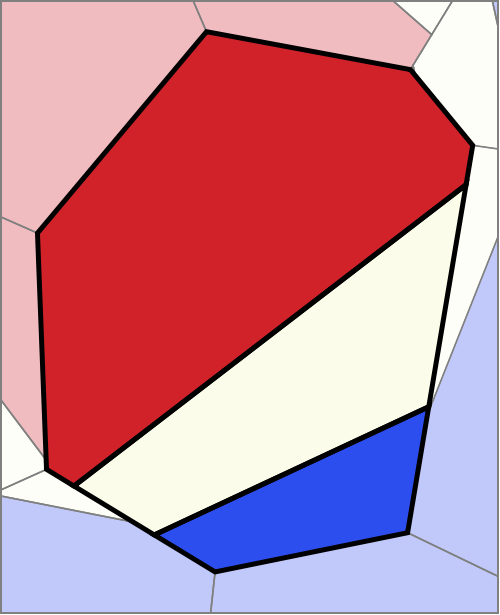
\includegraphics[width=0.3\textwidth]{./ring_mini_voronoi_cell.png}%{./Pictures/mainscreen1.png}
			\caption{Local polyhedral mesh for a three-material cell $T\in\bmesh$ \label{fig:mmesh}}
		\end{center}
		\vspace{-15pt}
		\vspace{1pt}
	\end{wrapfigure}
	If $T$ contains only one phase or material, then we obviously have $\mmesh(T) = \{\bcell\}$. Otherwise for the cell shared by several phases, $\mmesh(T)$ consists of polygonal elements, forming a tessellation of $T$, such that any ${\tau \in \mmesh(T)}$ contains only one phase/material; see Figure~\ref{fig:mmesh}. We denote by $\mfaces(T)$ the set of all faces in $\mmesh(T)$, which collects both   internal and boundary (external) faces with respect to $T$,  $\mfaces(T) = \mfaces[int](T) \cup \mfaces[ext](T)$. Thus for the example of local mesh drafted in Figure~\ref{fig:mmesh}, we have three elements in $\mmesh(T)$, two internal faces from $\mfaces[int](T)$ and eleven external faces from $\mfaces[ext](T)$. It is clear that this local mesh is fitted to the material interfaces.
	
	We shall discretize \eqref{dual_mini} in $T$ in terms of average fluxes assigned to each face from $\mfaces(T)$,
	we denote the corresponding vector by ${\vect u}_\mmesh\in\mathbb{R}^{n_f}$, $n_f=\#\mfaces(T)$,  and concentration values assigned to each cell ${\tau \in \mmesh(T)}$, we denote the corresponding vector by ${\vect p}_\mmesh\in\mathbb{R}^{n_p}$, $n_p=\#\mmesh(T)$. The given data is the source term vector ${\vect f}_\mmesh\in \mathbb{R}^{n_p}$ and the concentration values $\lambda$ on the boundary of $T$.
	To approximate this boundary data \emph{for the local problem}, we introduce the vector
	${\vect \lambda}_\mmesh\in\mathbb{R}^{n_\lambda}$, $n_\lambda=\#\mfaces[ext](T)$,
	where we assign one averaged concentration value for each $f\in\mfaces[ext](T)$, so that ${\vect \lambda}_\mmesh$ can be seen as a piecewise-constant approximation of $\lambda$ with respect to the subdivision of $\partial T$ into the faces of the local mesh $\mmesh$.
	
	%On the faces of macro mesh $\bmesh$ this
	
	Given the above definition of the degrees of freedom on the local mesh we apply the mimetic finite difference (MFD) method from~\cite{lipnikov2014mimetic}. The method leads to the following system of equations with the matrix having the block structure:
	\begin{equation}\label{local}
		\begin{pmatrix}
			\phantom{-}\vect M_\mmesh & \vect B^T_\mmesh \\
			-\vect B_\mmesh & \vect \Sigma_\mmesh
		\end{pmatrix}
		\begin{pmatrix}
			{\vect u}_\mmesh \\
			{\vect p}_\mmesh
		\end{pmatrix}
		=
		\begin{pmatrix}
			\vect E_\mmesh\,\vect C_\mmesh\,{\vect \lambda}_\mmesh \\
			{\vect f}_\mmesh
		\end{pmatrix}.
	\end{equation}
	Here $\vect M_\mmesh$, $\vect\Sigma_\mmesh$, $\vect B^T_\mmesh$, $-\vect B_\mmesh$ are vector-mass, mass, gradient and divergence matrices, respectively; $-\vect C_\mmesh$ is a diagonal scaling matrix, i.e. the mass matrix for ${\vect \lambda}_\mmesh$ unknowns;
	$\vect E_\mmesh \in \mathbb{R}^{n_f \times n_\lambda}$ is a rectangular matrix with 0 and 1 entries which sparsifies a vector from  $\mathbb{R}^{n_{\lambda}}$
	to a vector from  $\mathbb{R}^{n_{f}}$.
	For the details on MFD and accurate definition of the matrices we refer to \cite{lipnikov2014mimetic,MFDbook}.
	Here we need the property that  $\vect B_\mmesh$ has a full row rank, and $\vect M_\mmesh = \vect M^T_\mmesh$ is positive definite.
	
	Since the continuity of flux condition \eqref{flux_cond} and boundary conditions are enforced on  the \emph{external} edges of $T$, we need to distinct the vector ${\vect u}^\text{ext}_\mmesh$ of fluxes on $\mfaces[ext](T)$, which is just a trivial restriction of ${\vect u}_\mmesh$ on the edges  from $\mfaces[ext](T)$,
	\begin{equation}\label{system_mini}
		{\vect u}^\text{ext}_\mmesh \coloneqq \vect E_\mmesh^T\,{\vect u}_\mmesh,
	\end{equation}
	where $\vect E_\mmesh^T$ is the restriction matrix with entries equal $0$ or $1$.
	
	We now eliminate ${\vect u}_\mmesh$ from \eqref{local} and express ${\vect p}_\mmesh$ in terms of~${\vect \lambda}_\mmesh$ (\textit{static condensation}); recovering fluxes (backward substitution) and using~\eqref{system_mini} we get
	\begin{equation}\label{mini_flux_dofs}
		{\vect u}^\text{ext}_\mmesh = \vect A_\mmesh\,\vect C_\mmesh\,{\vect \lambda}_\mmesh - {\vect a}_\mmesh,
	\end{equation}
	with
	\begin{align} \label{defA}
		\vect A_\mmesh &= \vect E^T_\mmesh \left( \vect M^{-1}_\mmesh - \vect M^{-1}_\mmesh\,\vect B^T_\mmesh \left( \vect \Sigma_\mmesh + \vect B_\mmesh\,\vect M^{-1}_\mmesh\,\vect B^{T}_\mmesh\right)^{-1} \vect B_\mmesh\,\vect M^{-1}_\mmesh \right) \vect E_\mmesh, \\
		{\vect a}_\mmesh &= \vect E^{T}_\mmesh\,\vect M^{-1}_\mmesh\,\vect B^T_\mmesh \left( \vect \Sigma_\mmesh + \vect B_\mmesh\,\vect M^{-1}_\mmesh\,\vect B^{T}_\mmesh\right)^{-1} {\vect f}_\mmesh.
	\end{align}
	Note that matrices~$\vect A_\mmesh$ and vectors~${\vect a}_\mmesh$ are computed locally for each $T\in\bmesh$.
	\smallskip
	%	Matrix~$\vect A_\mmesh$ and vector~${\vect a}_\mmesh$ can be easily computed if the number of mini\,cells is relatively small. Otherwise, one may prefer to use a mixed-hybrid formulation instead of~$\eqref{weak_form}$ (see section~\ref{MH}).
	
	Next, we should use the continuity of flux condition \eqref{flux_cond} and boundary conditions to obtain a complete system for ${\vect u}^\text{ext}_\mmesh$ and ${\vect \lambda}_\mmesh$. However, we cannot do this in a straightforward way, since the discontinuity of material interfaces across the macro-mesh faces may lead to a mismatch of discrete fluxes from two sides of $F\in\bfaces[int]$, including different space dimensions.
	Therefore, we shall enforce the flux continuity condition in the spirit of the mortar finite element method~\cite{mortar} using the space of functions defined on $\bfaces[int]$, which are polynomials of degree at most $n$ on every $F\in\bfaces[int]$, an analog of the Lagrange multiplier space in the mortar method:
	\[
		\Lambda=\left\{\lambda\in \LTwoSpace[{\bfaces[int]}]\,:\, \lambda\in P_n~\text{for any}~F\in\bfaces[int]\right\}.
	\]
	
	%	Let $F \coloneqq {\bcell^+} \cap {\bcell^-}$, $F \in \bfaces[int]$, be a face shared by base\,cells~$\bcell^+$ and~${\bcell^- \in \bmesh}$ with mini\,meshes~$\mmesh^\pm$ and mini\,faces~$\mfaces^\pm$, respectively. We denote by~$\mfaces^\pm_F \subset \mfaces^\pm_{\text{ext}}$ mini\,faces that belong to the face~$F$. In general measures of mini\,faces of~$\mfaces^\pm_F$ corresponding to one material may be different, and, moreover, it may be the case that $\#\,\mfaces^+_F \ne \#\,\mfaces^-_F$ (see figure~\ref{fig:e_plus_e_minus}). That is, one may have different trace DOFs~\eqref{dual_mini:trace} from~$\mmesh^+$ and~$\mmesh^-$.
	%%	Let us set~$\nu_{F_{\bcell^\pm}} \coloneqq \#\,\mfaces^\pm_F$
	%	We set~$\nu_F \coloneqq \max\,\{ \#\,\mfaces^+_F,\,\#\,\mfaces^-_F \}$.
	%	
	%	\begin{figure}[h]
	%		\centering
	%		\caption{MMCs: $3 = \#\,\mfaces^+_F \ne \#\,\mfaces^-_F = 2$, $\nu_F = 3$}
	%		\label{fig:e_plus_e_minus}
	%		\svginputw[.7\linewidth]{e_plus_e_minus.pdf_tex}
	%	\end{figure}
	
	When the Lagrange multiplier space $\Lambda$ couples local MFD solutions, it is convenient to define
	degrees of freedom for $\lambda\in\Lambda$ in terms of its~$(n+1)$ moments $\lambda^{(i)}_F$ on every internal face $F\in\bfaces[int]$:
	\begin{equation}\label{asc_dofs}
		\lambda^{(i)}_F=\frac{\int_F  \lambda\,s_i \diff l}{|F|}, \quad i = 0, \dots, n.
	\end{equation}
	Here~$\{\,s_i\,\}_{i=0,\dots,n}$ is the set of $\LTwoSpace$-orthogonal polynomials on $F$ of degree~$n$.
	
	For $F \in \bfaces[int]$ shared by two polygonal cells~$\bcell^\pm\in \bmesh$  denote by~$\mfaces_F(T^\pm) \subset \mfaces_{\text{ext}}(T^\pm)$ the subsets of mini-faces that belong to the macro-face~$F$ from each side. Let $\nu_F \coloneqq \max\,\{ \#\,\mfaces_F(T^+),\,\#\,\mfaces_F(T^-) \}$. We set~$\bfaces_\bcell \subset \bfaces$ to be the subset of macro-faces forming the boundary of a cell~$T$. With each face $F \in \bfaces_\bcell$ we associate~$\min\,\{ n+1, \nu_F \}$ degrees of freedom~\eqref{asc_dofs} in the $\Lambda$ space. The local and global number of d.o.f. are
	\[
		n_\bcell \coloneqq \sum_{F \in \bfaces_\bcell} \min\,\{ n+1, \nu_F \} \quad\text{and}\quad
		n_\bmesh \coloneqq \sum_{F \in \bfaces} \min\,\{ n+1, \nu_F \},
	\]
	respectively.
	
	Further denote by~${{\vect \lambda}_\bcell \in \Rn{n_\bcell}}$ a vector of d.o.f. for elements of $\Lambda$ associated with all macro-faces spanning the boundary of~$\bcell$. We need a correspondence between elements of $\Lambda$ and local face elements $\vect \lambda_\mmesh$ used as boundary data in local problem \eqref{local}.
	This corresponding is given by the interpolation matrix $ \vect R_\mmesh$,
	\begin{equation}\label{asc_lambda}
		{\vect \lambda}_\mmesh = \vect R_\mmesh\,{\vect \lambda}_\bcell,
	\end{equation}
	where ${\vect \lambda}_\mmesh$ is effectively a piecewise constant approximation of ${\vect \lambda}_\bcell$ on $\mfaces_{\text{ext}}(T)$.
	Using this in \eqref{mini_flux_dofs}, we get
	\begin{equation}\label{asc_flux_lambda}
		{\vect u}^\text{ext}_\mmesh = \vect A_\mmesh\,\vect C_\mmesh\,\vect R_\mmesh\,{\vect \lambda}_\bcell - {\vect a}_\mmesh.
	\end{equation}
	%The interpolating matrix~$\vect R_\mmesh$ is completely defined by~$n$ and boundary mini\,faces~$\mfaces[ext]$ of~$\mmesh$.
	If we find the mortar vector ~${\vect \lambda}_\bcell$, we recover the local approximation to the face concentration, i.e. ${\vect \lambda}_\mmesh$, from~\eqref{asc_lambda}.
	Further we solve numerically local subproblems in~\eqref{dual_mini} applying the mimetic FD method. This completes the solution algorithm for \eqref{dual}.
	
	The dimension of the $\Lambda$ space is~$n_\bmesh$, i.e. $(n+1)$ or less unknowns for each face~${F \in \bfaces}$.
	To obtain the system of $n_\bmesh$ equations, we enforce the weak continuity of the moments of  fluxes  on each internal macro-face
	\begin{equation}\label{flux_cont}
		\int_F \vect u|_{\bcell^+}\cdot\hat{\vect n}\,s_i \diff l = \int_F \vect u|_{\bcell^-}\cdot\hat{\vect n}\,s_i \diff l, \quad i = 0, \dots, n, \quad \text{for each } F \in \bfaces[int],
	\end{equation}
	with $\big(\vect u|_{\bcell^+}\cdot\hat{\vect n}\big)(\vect x) = u^\text{ext}_\mmesh(f)\,|f|$, if $\vect x \in f$ for $f\in\mfaces_F(T^+)$, and $u^\text{ext}_\mmesh(f)$ is the local flux assigned to $f$ (component of~$\vect u^\text{ext}_\mmesh$). Similar definition applies to $\vect u|_{\bcell^-}$. 	
	This and~\eqref{asc_flux_lambda} result in the linear algebraic system
	\begin{equation}\label{asc_system}
		\vect S_\bmesh\,{\vect \lambda}_\bmesh = {\vect b}_\bmesh,
	\end{equation}
	with	$\vect S_\bmesh \in \Rn{n_\bmesh \times n_\bmesh}, {\vect \lambda}_\bmesh, {\vect b}_\bmesh \in \Rn{n_\bmesh}$.
	Neumann boundary condition in~\eqref{dual:bc} is handled in the similar way, and Dirichlet boundary data in~\eqref{dual:bc} is enforced strongly in~\eqref{asc_system}.
	
	Matrix~$\vect S_\bmesh$ is sparse and its sparsity pattern does not depend on mini-meshes. Some useful properties of this matrix will be discussed in the next section.
	
	\subsection{Matrix properties}
	
	In this section we discuss the assembly procedure of the global matrix from \eqref{asc_system} and show that $\vect S_\bmesh$ is symmetric positive definite. We concentrate on ASC(1), which we implement and validate  in the next section. We shall make necessary remarks about ASC(0) as it is largely obtained by obvious simplifications of ASC(1).
	
	\begin{figure}[h]
		\centering		
		\begin{subfigure}{.45\linewidth}
			\centering
			\svginputw{e_plus_1.pdf_tex}
			\caption{$\nu_F = 1$}%,
			\label{fig:asc_dofs:asc1:pc}
		\end{subfigure}%
		\qquad\quad
		\begin{subfigure}{.45\linewidth}
			\centering
			\svginputw{e_plus_2.pdf_tex}
			\caption{$\nu_F = 3$}		
		\end{subfigure}
		\caption{$\lambda_{ji}(\mmesh)$ are local d.o.f. used in MFD for $\lambda$ from \eqref{dual_mini}, $\lambda^{(0)}_j(T)$, $\lambda^{(1)}_j(T)$ are global d.o.f. used to describe mortar space $\Lambda$. Left: Face $F$ is single-material and uses one global d.o.f.; Right: Face $F$ is multi-material and uses two global d.o.f.
		\label{fig:asc_dofs:asc1:mmc}}
	\end{figure}
	
	The method uses local piecewise constant  and global piecewise $P_1$ \big(for ASC(1)\big) approximation of the concentration on $\bfaces$. Local piecewise constant approximations $\vect\lambda_\mmesh$, however, use finer local subdivisions, so $\vect\lambda_\mmesh$ does not belong to the restriction of the global space $\Lambda$ on the boundary of a given cell $T$. For the method, we define a mapping given by the matrix $\vect R_\mmesh$ to map global to local degrees of freedom and $\vect R_\mmesh^T$ from local   to global. For the well-posedness of the method, we need $\vect R_\mmesh$ to have a full rank.
	
	We define $\vect R_\mmesh$ locally for any fixed $\bcell\in\bmesh$. Let us enumerate all faces of the given $T$ by index $j$. For example, $j=1,\dots,4$ for the polygonal cell in Figure~\ref{fig:asc_dofs:asc1:mmc}. For each $j$, index $i$ enumerates mini-faces from $\mfaces[ext](T)$ belonging to the macro-face $j$. For example, $i\in\{1,2,3\}$ for $j=1$ and $i\in\{1\}$ for $j=4$ for the same example in Figure~\ref{fig:asc_dofs:asc1:mmc}. Further, denote by $\lambda_{j\,i}(\mmesh)$ the local d.o.f. assigned to the $i$-th mini-face belonging to the $j$-th macro-face, and by $\lambda^{(0)}_{j}(T)$, $\lambda^{(1)}_{j}(T)$ two moments defining an element from $\Lambda$ on the $j$-th macro-face (see Figure~\ref{fig:asc_dofs:asc1:mmc}) so that we have
	\begin{equation}\label{lambda_intermsof_moments}
		{\lambda}\big({\vect r}(t)\big) = \lambda^{(1)}_{j}(T)\,|F|\,t + \left( \lambda^{(0)}_{j}(T) - \frac{\lambda^{(1)}_{j}(T)\,|F|}{2} \right),\qquad  F\in\bfaces[int]
	\end{equation}
	for $\lambda\in\Lambda$. Here $t\in(0,1)$ and ${\vect r}\::\:\left(0,1\right) \rightarrow F$ is the affine parametrization of the face $F$ with index $j$ among macro-faces of $T$.
	
	Integrating \eqref{lambda_intermsof_moments} over all mini-faces $f \in \mfaces_\bface(\bcell)$ ($f$ has local index $i$ among mini-faces belonging to $F$) and re-scaling, we get
	\begin{equation}\label{asc1_interp}
		\lambda_{j\,i}(\mmesh) =
		\begin{cases}
			\lambda^{(0)}_{j}(\bcell) +  s_{j\,i}\,\lambda^{(1)}_{j}(\bcell), & \text{if}~F~\text{is a multi-material face}, \\
			\lambda^{(0)}_{j}(\bcell),                                        & \text{otherwise},
		\end{cases}
	\end{equation}
	where $s_{j\,i} $ is a signed distance between centroids of~$f$  and~$F$. For the corresponding vectors of unknowns  ${\vect \lambda}_\mmesh = \{ \lambda_{j\,i}(\mmesh) \}$ and ${\vect \lambda}_\bcell = \{ \lambda^{(0)}_{j}(\bcell) \} \cup \{ \lambda^{(1)}_{j}(\bcell) \}$ this defines
	the matrix $\vect R_\mmesh$ through~\eqref{asc_lambda}. For the example in Figure~\ref{fig:asc_dofs:asc1:mmc} (left and right) we have
	\begin{equation*}\footnotesize
		\vect R_\mmesh
		=
		\begin{pmatrix}
			1 &  s_{1\,1} & 0 & 0 & 0 & 0 & 0 \\
			1 &  s_{1\,2} & 0 & 0 & 0 & 0 & 0 \\
			1 &  s_{1\,3} & 0 & 0 & 0 & 0 & 0 \\
			0 & 0 & 1 &  s_{2\,1} & 0 & 0 & 0 \\
			0 & 0 & 1 &  s_{2\,2} & 0 & 0 & 0 \\
			0 & 0 & 1 &  s_{2\,3} & 0 & 0 & 0 \\
			0 & 0 & 0 & 0 & 1 &  s_{3\,1} & 0 \\
			0 & 0 & 0 & 0 & 1 &  s_{3\,2} & 0 \\
			0 & 0 & 0 & 0 & 0 & 0 & 1
		\end{pmatrix},
		\quad
		\vect \lambda_\mmesh = 
		\begin{pmatrix}
			\lambda_{11}(\mmesh) \\
			\lambda_{12}(\mmesh) \\
			\lambda_{13}(\mmesh) \\
			\lambda_{21}(\mmesh) \\
			\lambda_{22}(\mmesh) \\
			\lambda_{23}(\mmesh) \\
			\lambda_{31}(\mmesh) \\
			\lambda_{32}(\mmesh) \\
			\lambda_{41}(\mmesh) \\
		\end{pmatrix};	
	\end{equation*}
	for the moment d.o.f. we have
	\begin{align*}\footnotesize
		\vect \lambda_\bcell =& 
		\left(
			\lambda^{(0)}_1(\bcell),\,
			\lambda^{(1)}_1(\bcell),\,
			\lambda^{(0)}_2(\bcell),\,
			\lambda^{(1)}_2(\bcell),\,
			\lambda^{(0)}_3(\bcell),\,
			\lambda^{(1)}_3(\bcell),\,
			\lambda^{(0)}_4(\bcell)
		\right)^T
		\text{ and} \\
		&\left(
			\lambda^{(0)}_1(\bcell),\,
			\lambda^{(1)}_1(\bcell),\,
			\lambda^{(0)}_2(\bcell),\,
			\lambda^{(1)}_2(\bcell),\,
			\lambda^{(0)}_3(\bcell),\,
			\lambda^{(1)}_3(\bcell),\,
			\lambda^{(0)}_4(\bcell),\,
			\lambda^{(1)}_4(\bcell)
		\right)^T		
	\end{align*}
	for Figure~\ref{fig:asc_dofs:asc1:mmc} (left) and Figure~\ref{fig:asc_dofs:asc1:mmc} (right), respectively. For ASC(0) the matrix $\vect R_\mmesh$  is as above with rows containing $s_{ij}$-s eliminated.
	%Since the fourth base\,face $F \in \bfaces_\bcell$ has only one material, a trace on~$F$ from the cell~$\bcell$ is approximated by a constant. However, if in the adjacent cell we have several materials on $F$\footnotemark{}, we will use the value of~$\lambda'_{\bcell\,4}$ to improve the approximation of the fine traces on~$F$ in the adjacent cell.
	
	Now, when the mappings between local and global approximations of $\lambda$ are defined, we are ready to proceed with the assembly of the global matrix $\vect S_\bmesh$. The flux continuity over the face $F$ \big(condition~\eqref{flux_cont}\big) yields
	\begin{equation}\label{eq:aux1pre}
		\left\{\begin{split}
			\sum_{f\in \mfaces_F(T^+)} u^{\text{ext}}_{\mmesh^+}(f)\,|f| &+ \sum_{f\in \mfaces_F(T^-)} u^{\text{ext}}_{\mmesh^-}(f)\,|f| &= 0, \\
			\sum_{f\in \mfaces_F(T^+)} u^{\text{ext}}_{\mmesh^+}(f)\,\int_{f} s_1 \diff{l} &+ \sum_{f\in \mfaces_F(T^-)} u^{\text{ext}}_{\mmesh^-}(f)\,\int_{f} s_1 \diff{l} &= 0
		\end{split}\right.
		%\quad\Leftrightarrow \\
		%		\sum_{i \in I_{\mfaces^+_F}} u^{\text{ext}}_{\mmesh^+\,i}\,\Delta s^+_i\,|\mfaces^+_{F\,i}| &+ \sum_{i \in I_{\mfaces^-_F}} u^{\text{ext}}_{\mmesh^-\,i}\,\Delta s^-_i\,|\mfaces^-_{F\,i}| = 0,
	\end{equation}
	or in the matrix form
	\begin{equation}\label{eq:aux1}
		\left( \vect R^T_{\mmesh^+}\,\vect C_{\mmesh^+}\,{\vect u}^{\text{ext}}_{\mmesh^+} \right)_{i+m} + \left( \vect R^T_{\mmesh^-}\,\vect C_{\mmesh^-}\,{\vect u}^{\text{ext}}_{\mmesh^-} \right)_{j+m} = 0, \quad m \in \{0, 1\}
	\end{equation}
	where $i$ and $j$ are the local indexes of the face $F$ in the cells $T^+$ and $T^-$, respectively. ($m = 0$ corresponds to the first equation in~\eqref{eq:aux1pre} and $m = 1$ corresponds to the second one; further we omit ``$+m$" for simplicity.) For the Neumann part of the boundary of~$\bcell^\pm$ we set $\mfaces_N(\bcell^\pm) \coloneqq \{ f \in \mfaces[ext](\bcell^\pm)\::\:f \subset \partial\Omega_N \}$. If $F$ from $T^+$ belongs to the Neumann part of the boundary, then we have
	\begin{equation*}
		\left( \vect R^T_{\mmesh^+}\,\vect C_{\mmesh^+}\,{\vect u}^{\text{ext}}_{\mmesh^+} \right)_i = \left( \vect R^T_{\mmesh^+}\,\vect C_{\mmesh^+}\,{\vect g}_{N\,\mmesh^+} \right)_i, \quad
		{\vect g}_{N\,\mmesh^+} \coloneqq \left\{ \int_f g_N\,s_k \diff{l}\,/\,|f| \right\}_{f\,\in\,\mfaces_N(\bcell^+),\:k\,\in\,\{0,\,1\}}.
	\end{equation*}
	
	Substituting~\eqref{asc_flux_lambda} into \eqref{eq:aux1} we get the local equation for~${\vect \lambda}_\bcell$
	\begin{align}\label{local_system}
		\begin{split}
			\Big( \underbrace{\left( \vect R^T_{\mmesh^+}\,\vect C_{\mmesh^+}\,\vect A_{\mmesh^+}\,\vect C_{\mmesh^+}\,\vect R_{\mmesh^+} \right)}_{\vect S_{\bcell^+} \coloneqq} {\vect \lambda}_{\bcell^+} \Big)_i
			&+
			\Big( \underbrace{\left( \vect R^T_{\mmesh^-}\,\vect C_{\mmesh^-}\,\vect A_{\mmesh^-}\,\vect C_{\mmesh^-}\,\vect R_{\mmesh^-} \right)}_{\vect S_{\bcell^-} \coloneqq} {\vect \lambda}_{\bcell^-} \Big)_j = \\
			\big( \underbrace{\vect R^T_{\mmesh^+}\,\vect C_{\mmesh^+}\,{\vect a}_{\mmesh^+}}_{{\vect b}_{\bcell^+} \coloneqq} \big)_i
			&+
			\big( \underbrace{\vect R^T_{\mmesh^-}\,\vect C_{\mmesh^-}\,{\vect a}_{\mmesh^-}}_{{\vect b}_{\bcell^-} \coloneqq} \big)_j.
		\end{split}
	\end{align}
	As standard in finite element methods, one assembles the global system~\eqref{asc_system} from the local matrices and local right-hand side vectors.  Thus we may formally write
	\begin{align}\label{global_system_assembly}
		%\begin{split}
		\vect S_\bmesh = \sum_{\bcell \in \bmesh} \vect N^T_\bcell\,\vect S_\bcell\,\vect N_\bcell, \quad
		{\vect b}_\bmesh = \sum_{\bcell \in \bmesh} \vect N^T_\bcell\,{\vect b}_\bcell,
		%\end{split}
	\end{align}
	where $\vect N_\bcell$ defines global to local mapping for the cell $T$.
	
	From~\eqref{local_system} it is clear that~$\vect S_\bmesh$ is sparse: Global d.o.f. $\lambda^{(0)}_m(\bmesh)$, $\lambda^{(1)}_m(\bmesh)$ (components of~$\vect\lambda_\bmesh$) interact only with d.o.f. associated with faces of macro-cells that share $m$th macro-face. For example, if $F\in\bfaces[int]$ is shared by two quadrilaterals and has global index $m$, then $m$th row of~$\vect S_\bmesh$ has at most 14 nonzero elements for ASC(1) and at most 7 for ASC(0). %; if $i$th base\,face is a face shared by a quadrilateral and a triangle, $i$th row of~$\vect S_\bmesh$ will have~6 nonzero elements and so forth.
	
	Now we show that the global matrix~$\vect S_\bmesh$ in~\eqref{asc_system} is symmetric and positive definite. We give the arguments for ASC(1). Same arguments hold for ASC(0) after obvious simplifications.
	\vskip .2cm
	%\begin{theorem}\label{thm:asc0}
	%		$\Ker\vect R_\mmesh = \{ {\vect 0} \}$ for ASC(0)
	%	\end{theorem}
	%	\begin{proof}
	%		From~\eqref{asc0_interp} we have that for any cell~$\bcell$\,/\,its mini\,mesh~$\mmesh$ the interpolating matrix may be written as
	%		\begin{equation*}
	%			\vect R_\mmesh =
	%			\begin{pmatrix}
	%				{\vect e}_1 & & & \\
	%				& {\vect e}_2 & & \\
	%				& & \ddots & \\
	%				& & & {\vect e}_m
	%			\end{pmatrix},
	%		\end{equation*}
	%		where~$m \coloneqq$ number of base\,faces spanning~$\bcell$ and ${\vect e}_k \coloneqq$ column vector of all ones; its length is the number of mini\,faces of the base\,face~$k$. Clearly, columns of~$\vect R_\mmesh$ are linearly independent.
	%		
	%	\end{proof}
	\begin{lemma}\label{thm:asc1}
		%If~$\bfaces_\bcell \cap \bfaces[\textnormal{mixed}] = \varnothing$, then~
		$\Ker\vect R_\mmesh = \{ {\vect 0} \}$ for ASC(1)
	\end{lemma}
	\begin{proof}
		\vskip -.3cm
		From~\eqref{asc1_interp} we have that for any cell~$\bcell$ and its mini-mesh~$\mmesh(T)$
		%that has no mixed base\,faces, ${\bfaces_\bcell \cap \bfaces[mixed] = \varnothing}$,
		the interpolating matrix may be written as
		\begin{equation}\label{r_wo_mixed}\footnotesize
			\vect R_\mmesh =
			\begin{pmatrix}
				\vect S_1 & & & \\
				& \vect S_2 & & \\
				& & \ddots & \\
				& & & \vect S_m
			\end{pmatrix},
		\end{equation}
		where~$m \coloneqq$ number of macro-faces spanning~$\partial\bcell$ and
		\begin{equation*}
			\vect S_k \coloneqq
			\begin{cases}
				\begin{pmatrix}
					1 &  s_{k\,1} \\
					\vdots & \vdots \\
					1 &  s_{k\,m_k} \\
				\end{pmatrix}, & \text{if }k\text{th face is multi-material face}, \\
				1, & \text{otherwise},
			\end{cases}
		\end{equation*}
		$1 < m_k$ is the number of mini-faces of the~$k$th macro-face, $ s_{k\,i}$ is the signed distance between centroids of~$i$th mini-face and~$k$th macro-face. If~$\bcell$ contains only one material, then $\vect R_\mmesh = \vect I$ and hence $\Ker\vect R_\mmesh = \{ {\vect 0} \}$, so we assume that there is at least one multi-material  face.
		
		Clearly, matrix~$\vect R_\mmesh$ has a non-trivial kernel iff
		\begin{equation*}
			s_{k\,i} =  s_{k\,j}, \quad i, j = 1, 2, \dots, m_k
		\end{equation*}
		for some~$k$. Take some $\vect S = \vect S_k$ corresponding to a multi-material face~$F \in \bfaces_\bcell$ with~${l \coloneqq m_k}$ materials,
		\begin{equation*}
			\vect S = \begin{pmatrix}
				1 &  s_1 \\
				\vdots & \vdots \\
				1 &  s_l \\
			\end{pmatrix}.
		\end{equation*}
		It is sufficient to show that~$ s_1 \ne  s_2$. Let $f_1$ and $f_2$ be corresponding mini-faces. We have
		\[
			s_1 = \frac{1}{2}\left( |f_1| - |F| \right), \quad
			s_2 = |f_1| + \frac{1}{2}\left( |f_2| - |F| \right),
		\]
		and
		\begin{equation*}
			s_1 =  s_2 \quad\Leftrightarrow\quad |f_1| + |f_2| = 0.
		\end{equation*}
		Hence $ s_1 \ne  s_2$, and~$\Ker\vect R_\mmesh = \{ {\vect 0} \}$ follows.
	\end{proof}
	\vskip .3cm
	\begin{theorem}
		Matrix $\vect S_\bmesh$ is symmetric. If $c > 0$ or $|\partial\Omega_D|>0 $, then  $\vect S_\bmesh$ is positive definite.
	\end{theorem}
	\begin{proof}
		\vskip -.3cm
		First, noting that for any two symmetric positive definite matrices $\vect A_1$ and $\vect A_2$ inequality $\vect A_1 \ge \vect A_2$ implies $\vect A_1^{-1} \le \vect A_2^{-1}$, we conclude
		\begin{equation}\label{aux2}
			\widetilde{\vect B}^T \left( \vect \Sigma+ \widetilde{\vect B}\,\widetilde{\vect B}^{T}\right)^{-1} \widetilde{\vect B}
			\le
			\widetilde{\vect B}^T \left(\widetilde{\vect B}\,\widetilde{\vect B}^{T}\right)^{-1} \widetilde{\vect B} \le \vect I,
		\end{equation}
		where $\vect \Sigma$ is any symmetric and non-negative definite matrix, $\widetilde{\vect B}$ is any matrix such that \\ ${\Ker\widetilde{\vect B}^T = \{ \vect 0 \}}$, and $\vect I$ is identity matrix. To check the last inequality in~\eqref{aux2}, one can consider, e.g., the SVD decomposition of $\widetilde{\vect B}$.
		
		From the identities~\eqref{defA} and~\eqref{aux2} with $\widetilde{\vect B}^T \coloneqq \vect M^{-\frac12}_\mmesh\,\vect B_\mmesh^T$, $\vect \Sigma \coloneqq \vect \Sigma_\mmesh$ it immediately follows that $\vect A_{\mmesh}$ is symmetric and non-negative definite.  The symmetry of $\vect S_\bmesh$ follows from the definition in \eqref{local_system}--\eqref{global_system_assembly}.
		By similar considerations, it is easy to see that $\vect A_{\mmesh}$ is positive definite for all~$\bcell$, where $c > 0$. Hence if $c > 0$ in $\Omega$ , then \eqref{local_system}--\eqref{global_system_assembly} and the full ranks of $\vect R_\mmesh$'s and $\vect C_\mmesh$'s imply
		the positive definiteness of $\vect S_\bmesh$.
		
		Now we show the positive definiteness of $\vect S_\bmesh$ if $|\partial\Omega_D|>0 $. Consider  any given $\bcell\in\bmesh$.
		Matrix  $\vect A_{\mmesh}$ defines the discrete Dirichlet-to-Neumann map for $\partial\bcell$.
		If $\partial\bcell\cap\partial\Omega_D$, then $\Ker \vect A_{\mmesh} = \{\vect 0\}$. Otherwise $\Dim\big(\Ker \vect A_{\mmesh}\big) = 1$ and $\vect A_{\mmesh}\,\vect C_{\mmesh}\,\vect\lambda_\mmesh=0$ implies that $\vect\lambda_\mmesh$ is constant on $\partial\bcell$. Consider some $\lambda$ from the mortar space $\Lambda$ and corresponding vector of moments  $\vect \lambda_\bmesh$. Using connectivity of the mesh one easily finds that $\vect R_\mmesh\,\vect\lambda_\bcell$ can be constant on every $T\in\bmesh$ only if $\lambda$ is constant. Due to the assumption $|\partial\Omega_D|>0$ this implies $\lambda=0$.
		% Thus we have
		%		\begin{equation*}
		%			\big(\vect S_\bcell\,{\vect x},\,{\vect x}\big) =
		%			\big(\vect R^T_\mmesh \left( \vect C_{\mmesh}\,\vect A_{\mmesh}\,\vect C_{\mmesh} \right) \vect R_\mmesh\,{\vect x},\,{\vect x} \big) =
		%			\big(\vect A_{\mmesh}\,\vect C_{\mmesh}\,\vect R_\mmesh\,{\vect x},\,\vect C_{\mmesh}\,\vect R_\mmesh\,{\vect x} \big) \ge 0
		%		\end{equation*}
		%		for all~$\bcell \in \bmesh$ and
		%		\begin{equation*}
		%			\big(\vect S_\bcell\,{\vect x},\,{\vect x} \big) > 0
		%		\end{equation*}
		%		for some~$\bcell \in \bmesh$ since~$\Ker\vect R_\mmesh = \{ {\vect 0} \}$. So
		Hence for any $\vect0\neq\vect\lambda_\bmesh\in \mathbb{R}^{n_\bmesh}$ we have
		\begin{align*}
		\left(\vect S_\bmesh\,\vect\lambda_\bmesh,\,\vect\lambda_\bmesh\right) &\stackrel{\eqref{global_system_assembly}}{=}
		\Big( \big( \sum_{\bcell \in \bmesh} \vect N^T_\bcell\,\vect S_\bcell\,\vect N_\bcell \big){\vect\lambda_\bmesh},\,{\vect\lambda_\bmesh} \Big) =
		\sum_{\bcell \in \bmesh} \big( \vect S_\bcell\,\vect N_\bcell\,{\vect\lambda_\bmesh},\,\underbrace{\vect N_\bcell\,{\vect\lambda_\bmesh}}_{{\vect \lambda_\bcell} =} \big) \\
		& = \sum_{\bcell \in \bmesh} \big(\vect S_\bcell\,{\vect \lambda_\bcell},\,{\vect \lambda_\bcell} \big) > 0.
		\end{align*}
		The last inequality holds, since there exists $\bcell$ such that $\vect \lambda_\bcell=\vect N_\bcell\,{\vect\lambda_\bmesh}$ is not in the kernel for $\vect\lambda_\bmesh\neq\vect0$.
	\end{proof}

	\section{Numerical Results}\label{sec:num}

Let $h$ be a max cell diameter for the macro-mesh~$\bmesh_h$, and $\mathbb V_h \subset \LTwoSpace$ be a space of piecewise constant
functions on each cell~$\mcell \in \mmesh(\bcell)$, $\bcell \in \bmesh_h$. We define \textit{discrete} $\LTwo$-norm of $v \in \LTwoSpace$ as
\begin{equation}\label{l2}
  \| v \|_{\lTwoSpace} \coloneqq \| P_h\,v \|_{\LTwoSpace},
\end{equation}
where $P_h\;:\;\LTwoSpace\rightarrow\mathbb V_h$ is $\LTwo$-projection operator.

For the error~$e_h \coloneqq p - p_h$ between the exact and computed solutions we have
\begin{equation}\label{l2norm}
	\errlTwo{h} \coloneqq \| e_h \|_{\lTwoSpace} = \| p - p_h \|_{\lTwoSpace} = \| P_h\,p - P_h\,p_h \|_{\LTwoSpace} = \| P_h\,p - p_h \|_{\LTwoSpace}
\end{equation}
since~$P_h$ is linear and~$p_h \in \mathbb V_h$. The discrete norm~\eqref{l2norm} of the discretization error is computed as follows:
$$
	\errlTwo{h} = \left[\sum\limits_{\bcell \in \bmesh_h}\sum\limits_{\mcell\in\mmesh(\bcell)} \left(\frac{1}{|\mcell|}\int_{\mcell} p \diff{\vect x} - p_h(\mcell)\right)^2|\mcell|\right]^\frac12,
$$
where $|\mcell|$ is the area of cell $\mcell$.

If~$\bmesh_h$ consists of triangles and no material interfaces are present, ASC($n$) boils down to mixed-hybrid Raviart\,--\,Thomas finite element method (which is algebraically equivalent to~$R\,T_0$ finite element method). In this particular case we have~\cite{M2AN_1980__14_3_249_0}
$$
	\|\vect u - \vect u_h\|_{\LTwoSpace} \le c\,h\,\|\vect u\|_{\HSpace{1}},\quad\|p - p_h\|_{\LTwoSpace} \le c \left( h\,\|p\|_{\HSpace{1}} + h^2\,\|p\|_{\HSpace{2}} \right),
$$
so one cannot expect ASC($n$) $\LTwo$-convergence to be better than linear. Note that
\begin{equation}\label{l2L2}
	\| p - p_h \|_{\lTwoSpace} \le \| p - p_h \|_{\LTwoSpace}
\end{equation}
since $\| p - p_h \|_{\lTwoSpace} = \| P_h\,(p - p_h) \|_{\lTwoSpace} \le \|P_h\|_{\mathcal L(\LTwoSpace, \mathbb V_h)} \| p - p_h \|_{\LTwoSpace}$, and the operator norm~$\|P_h\|_{\mathcal L(\LTwoSpace, \mathbb V_h)} = 1$ by Pythagorean theorem. Thus one may expect some improvement in $\lTwo$-convergence as one increases~$n$ for ASC($n$).  

\subsection{Linear solution}

\begin{figure}[h]
	\centering
	\begin{subfigure}{.41\linewidth}
		\centering
		\includegraphicsw{err2_asc0.png}
		\caption{$\vect K_1 \equiv \vect K_2 \equiv \vect I$}
		\label{fig:fake:2}
	\end{subfigure}%
	\hfill
	\begin{subfigure}{.41\linewidth}
		\centering
		\includegraphicsw{err3_asc0.png}
		\caption{$\vect K_1 \equiv \vect K_2 \equiv \vect K_3 \equiv \vect I$}
		\label{fig:fake:3}
	\end{subfigure}
	\caption{Material distribution for pseudo-multi-material problem: two materials (left), three materials (right)
	\label{fig:fake}}		
\end{figure}

The first set of tests is designed to check the property of the method to accurately recover the solution that is the polynomial of degree~1. Let us consider the diffusion problem~\eqref{dual} with~$c \equiv f \equiv 0$, $\partial\Omega_D = \partial\Omega$. The computational domain $\Omega=(0,1)^2$ is divided into several subdomains by non-intersecting straight lines. In these settings the interface reconstruction algorithm MOF reconstructs the interfaces exactly. To test the {\it linearity preservation} property, we set up a pseudo-multi-material problem with the diffusion tensor being the same in all subdomains, $\vect K_i = \vect I$. The exact solution a linear function. The geometry of two cases under consideration is shown in Figure~\ref{fig:fake}.
	
We denote the solution computed  with the ASC($n$) method by~$p_{h,\,n}$, $n = 0, 1$. For ASC(0) we have~$\errlTwo{h,\,0} = 6.38 \times 10^{-2}$ and $6.41 \times 10^{-2}$ for the configurations shown in Figures~\ref{fig:fake:2} and~\ref{fig:fake:3}, respectively. That is, ASC(0) is not able to recover $P_1$ solutions exactly.

Since ASC(1) approximates interface traces with $P_1$ functions it recovers edge-based degrees of freedom exactly in the sense of mean values. This results in exact reconstruction of cell-based unknowns and {\it linearity preservation} property for both examples, i.e.
\begin{equation*}
	\errlTwo{h,\,1} = \left\| p - p_{h,\,1} \right\|_{\lTwoSpace} = 0.
\end{equation*}
% As we saw in previous section,
%In general, one may not expect concentration and flux convergence to be better than second order with respect to~$\lTwo$\,--\,error for ASC($1$).  However, taking the example above into account, one may expect that convergence of ASC(1) with respect to~$\lTwo$-norm is superior
%to  convergence properties of ASC(0).

\subsection{Piecewise $P_1$ solution}

In this set of tests, we consider the diffusion problem~\eqref{dual} with~$c \equiv f \equiv 0$, $\partial\Omega_D = \partial\Omega$, and two different materials in the domain. $\vect K = k\,\vect I$, $k = 1$ in the left part of the domain and $k = 0.1$ in the right (see Figure~\ref{fig:pwlin:mat}). The exact solution is piecewise linear such that the normal flux is continuous across the interface (see Figure~\ref{fig:pwlin:p}).
	
\begin{figure}[h!]
	\centering
	\label{fig:pwlin}
	\begin{subfigure}{.44\linewidth}
		\centering
		\includegraphicsw{skew_ref.png}
		\caption{Reference solution~$p$}
		\label{fig:pwlin:p}
	\end{subfigure}%
	\hfill
	\begin{subfigure}{.4\linewidth}
		\centering
		\includegraphicsw{skew_geometry_square.png}
		\caption{Materials: $k_1 = 1$, $k_2 = 0.1$}
		\label{fig:pwlin:mat}
	\end{subfigure}
	\caption{Piecewise linear reference solution}
\end{figure}

For this example we use a sequence of square base\,meshes~$\bmesh_{h_i}$, $i = 1, 2, 3, 4$. We denote by
\begin{equation*}
	\rho_{h_i,\,n} \coloneqq \frac{\ln \errlTwo{h_i,\,n} / \errlTwo{h_{i+1},\,n}}{\ln h_i / h_{i+1}}
\end{equation*}
the reduction rate order of ASC($n$) in~$\lTwo$-norm between $i$th and $(i+1)$th refinement steps. We also compute the $\ell^{\infty}$-norm of the error
\begin{equation*}
	\errInf{h_i,\,n} \coloneqq \left\| p - p_{h_i,\,n} \right\|_\infty
\end{equation*}
for ASC($n$).
	
\begin{table}[h!]
	\centering
	\caption{Piecewise linear example: convergence \label{fig:conv:pwlin}}
	\footnotesize
	\begin{tabular}[1.5]{| c | c || c | c || c |}
		\hline
		\multirow{5}{*}{\rotatebox{90}{ASC(0)}} & $h$ & $\errlTwo{0}$ & $\rho$ & $\errInf{0}$ \\
		\cline{2-5}
		& $3.5\times10^{-1}$ & $7.3\times10^{-1}$ & & 4.8 \\
		\cline{2-5}
		& $8.8\times10^{-2}$ & $1.6\times10^{-1}$ & 1.1 & 1.2 \\
		\cline{2-5}
		& $2.2\times10^{-2}$ & $3.7\times10^{-2}$ & 1.1 & $3.4\times10^{-1}$ \\
		\cline{2-5}
		& $5.5\times10^{-3}$ & $8.9\times10^{-3}$ & 1.0 & $7.9\times10^{-2}$ \\
		\hline
		\hline
		\multirow{5}{*}{\rotatebox{90}{ASC(1)}} & $h$ & $\errlTwo{1}$ & $\rho$ & $\errInf{1}$ \\
		\cline{2-5}
		& $3.5\times10^{-1}$ & $2.5\times10^{-2}$ & & $1.6\times10^{-1}$ \\
		\cline{2-5}
		& $8.8\times10^{-2}$ & $1.9\times10^{-3}$ & 1.84 & $6.3\times10^{-2}$ \\
		\cline{2-5}
		& $2.2\times10^{-2}$ & $1.6\times10^{-4}$ & 1.79 & $9.8\times10^{-3}$ \\
		\cline{2-5}
		& $5.5\times10^{-3}$ & $1.3\times10^{-5}$ & 1.80 & $4.0\times10^{-3}$ \\
		\hline
	\end{tabular}
\end{table}

Numerical results are shown in Table~\ref{fig:conv:pwlin}. We observe that ASC(0) converges linearly with respect to the $\lTwo$-norm, and ASC(1) has the convergence rate close to quadratic with respect to the $\lTwo$-norm.

\subsection{Piecewise $P_2$ solutions}
	
\subsubsection{Two materials}\label{sec:twomat}

\begin{figure}[h]
	\begin{subfigure}{.45\linewidth}
		\centering
		\includegraphicsw{circle_ref_mesh.png}
		\caption{Reference solution~$p$}
	\end{subfigure}%
	\hfill
	\begin{subfigure}{.45\linewidth}
		\centering
		\includegraphicsw{circle_ref_slice.png}
		\caption{$p(x,\frac{1}{2})$}
	\end{subfigure}
	\caption{Piecewise quadratic reference solution, 2 materials\label{fig:pwquad2}}
\end{figure}

Let us consider the diffusion problem~\eqref{dual} with~$c \equiv 0$, $\partial\Omega_D = \partial\Omega$. The computational domain is divided into subdomains: $\Omega_1 = \{ {\bf x} : \|{\bf x} - {\bf x}_0\|< 0.2\}$ with~${\bf x}_0 = (0.5,0.5)$ and $\Omega_2 = (0,1)^2 \setminus \bar{\Omega}_1$. The diffusion tensor is set to be $\vect K_i = k_i\,\vect I$ in $\Omega_i$, $k_1 = 0.001$ and $k_2=1$. The exact solution is piecewise quadratic such that the normal flux is continuous across the interface (see Figure~\ref{fig:pwquad2}). For this problem we compare convergence properties of the  ASC(0) and ASC(1) methods on a sequence of Voronoi meshes.

\begin{table}[h!]
	\centering
	\caption{Piecewise quadratic example, two materials: convergence \label{tab:conv:pwquad2}}
	\footnotesize
	\begin{tabular}[1.1]{| c | c || c | c || c |}
		\hline
		\multirow{7}{*}{\rotatebox{90}{ASC(0)}} & $h$ & $\errlTwo{0}$ & ${\rho}$ & $\errInf{0}$ \\
		\cline{2-5}
		& $3.0\times10^{-1}$ & $2.4\times10^{-3}$ & & $6.3\times10^{-1}$ \\
		\cline{2-5}
		& $1.5\times10^{-1}$ & $6.5\times10^{-4}$ & 2.0 & $7.0\times10^{-3}$ \\
		\cline{2-5}
		& $8.1\times10^{-2}$ & $2.6\times10^{-4}$ & 1.4 & $3.2\times10^{-3}$ \\
		\cline{2-5}
		& $4.2\times10^{-2}$ & $1.4\times10^{-4}$ & 0.9 & $2.3\times10^{-3}$ \\
		\cline{2-5}
		& $2.1\times10^{-2}$ & $3.7\times10^{-5}$ & 1.9 & $1.1\times10^{-3}$ \\
		\cline{2-5}
		& $1.0\times10^{-2}$ & $2.7\times10^{-5}$ & 0.4 & $8.6\times10^{-4}$ \\
		\hline
	\end{tabular}
	\begin{tabular}[1.1]{| c | c || c | c || c |}
		\hline
		\multirow{7}{*}{\rotatebox{90}{ASC(1)}} & $h$ & $\errlTwo{1}$ & ${\rho}$ & $\errInf{1}$ \\
		\cline{2-5}
		& $3.0\times10^{-1}$ & $2.4\times10^{-3}$ & & $2.1\times10^{-3}$ \\
		\cline{2-5}
		& {$1.5\times10^{-1}$} & $7.0\times10^{-4}$ & 1.9 & {$1.3\times10^{-2}$} \\
		\cline{2-5}
		& $8.1\times10^{-2}$ & $2.3\times10^{-4}$ & 1.8 & $6.8\times10^{-4}$ \\
		\cline{2-5}
		& $4.2\times10^{-2}$ & $6.8\times10^{-5}$ & 1.8 & $3.2\times10^{-4}$ \\
		\cline{2-5}
		& $2.1\times10^{-2}$ & $2.0\times10^{-5}$ & 1.8 & $1.1\times10^{-4}$ \\
		\cline{2-5}
		& $1.0\times10^{-2}$ & $5.4\times10^{-6}$ & 1.9 & $3.3\times10^{-5}$ \\
		\hline
	\end{tabular}
\end{table}

The norms of the errors are shown in Table~\ref{tab:conv:pwquad2}. ASC(1) demonstrates convergence with the rate in the $\lTwo$-norm close to quadratic. ASC(0) convergence rate fluctuates significantly.

We also observe a bump in the max norm error for ASC(1) on the second mesh level, $h = 1.5\times10^{-1}$. To have some insight, we show the corresponding mesh in the Figure~\ref{fig:conv:pwquad2:inf:mesh}. One may note that the interface reconstruction produces significant discontinuity of interfaces: A small volume of the external material, i.e. the one occupying $\Omega_2$ domain, appears inside the disk (domain $\Omega_1$). Due to constant trace approximation, ASC(0) is not sensitive to such irregularity. It turns out that for ASC(1) the $\ell^\infty$ norm of the error is affected by the appearance of such small isolated cut cells. At the same time, this does not affect the $\lTwo$-convergence of ASC(1).

\begin{figure}[h]
	\centering
	\label{fig:conv:pwquad2:inf}
	\begin{subfigure}{.29\linewidth}
		\centering
		\includegraphicsw{circle_voronoi_2_mat.png}
		\caption{Materials}
		\label{fig:conv:pwquad2:inf:mesh}
	\end{subfigure}%
	\hskip .6cm
	\begin{subfigure}{.33\linewidth}
		\centering
		\includegraphicsw{circle_voronoi_2_asc0.png}
		\caption{ASC(0), $p_h$}
	\end{subfigure}%
	\hskip1ex
	\begin{subfigure}{.33\linewidth}
		\centering
		\includegraphicsw{circle_voronoi_2_asc1.png}
		\caption{ASC(1), $p_h$}			
	\end{subfigure}%
	\caption{Piecewise quadratic example, two materials: $h = 1.5\times10^{-1}$. This figure illustrates the appearance of small isolated material volumes during numerical reconstruction of material interfaces. This may affect the $\ell^\infty$ error norm of the ASC(1)}
\end{figure}

\subsubsection{Three materials}\label{sec:threemat}

\begin{figure}[h]
	\centering
	\begin{subfigure}{.45\linewidth}
		\centering
		\includegraphicsw{ring_ref_mesh.png}
		\caption{Reference solution~$p$}
	\end{subfigure}%
	\hfill
	\begin{subfigure}{.45\linewidth}
		\centering
		\includegraphicsw{ring_ref_slice.png}
		\caption{$p(x,\frac{1}{2})$}
	\end{subfigure}
	\caption{Piecewise quadratic reference solution, three materials \label{fig:pwquad3}}
\end{figure}
		
In the next group of numerical tests, we consider the same  diffusion problem~\eqref{dual} with~$c \equiv 0$, $\partial\Omega_D = \partial\Omega$. The computational domain is now divided into three subdomains: $\Omega_1 = \{{\bf x} : \|{\bf x} - {\bf x}_0\| < 0.15\}$, $\Omega_2 = \{{\bf x} : 0.15 < \|{\bf x} - {\bf x}_0\| < 0.2\}$, and $\Omega_3 = (0,1)^2 \setminus (\bar{\Omega}_1\cup\bar{\Omega}_2)$. The diffusion tensor is set to be $\vect K_i = k_i\,\vect I$, $k_{1} = k_{3} = 1$, $k_2 = 0.001$. The geometry represents a ring with $k_2=0.001$ inside the ring and $k_{1} = k_{3} = 1$ outside the ring. The exact solution is piecewise quadratic such that the normal flux is continuous across the interface; see Figure~\ref{fig:pwquad3}. We use a sequence of triangular meshes to study convergence for this example. In this set of tests, we also consider the numerical method based on homogenization techniques for the comparison. The homogenization method we use is from \cite{dawes2013solving}. The homogenized values of the diffusion tensor are computed on the base cells $\bcell$ and then plugged into the MFD discretization applied on the  base mesh $\bmesh_h$; see \cite{kikinzon2017approximate} for implementation details of this method.

\begin{table}[h]
	\centering
	\caption{Piecewise quadratic example, three materials: error norms and convergence rates\label{fig:conv:pwquad3}}
	\footnotesize
	\begin{tabular}[1.1]{| c | c || c | c || c |}
		\hline
		\multirow{7}{*}{\rotatebox{90}{ASC(0)}} & $h$ & $\errlTwo{0}$ & $\rho$ & $\errInf{0}$ \\
		\cline{2-5}
		& $3.0\times10^{-1}$ & 4.5 & & 17 \\
		\cline{2-5}
		& $2.5\times10^{-1}$ & 4.5 & & 17 \\
		\cline{2-5}
		& $1.3\times10^{-1}$ & 4.0 & & 17 \\
		\cline{2-5}
		& $8.3\times10^{-2}$ & 4.4 & & 17 \\
		\cline{2-5}
		& {$6.7\times10^{-2}$} & $7.1\times10^{-1}$ & & 4.9 \\
		\cline{2-5}
		& $4.3\times10^{-2}$ & $4.5\times10^{-1}$ & 1.2 & 5.0 \\
		\hline
		\hline
		\multirow{7}{*}{\rotatebox{90}{ASC(1)}} & $h$ & $\errlTwo{0}$ & $\rho$ & $\errInf{0}$ \\
		\cline{2-5}
		& $3.0\times10^{-1}$ & $4.5\times10^{-1}$ & & 3.5 \\
		\cline{2-5}
		& $2.5\times10^{-1}$ & $2.6\times10^{-1}$ & 3 & 2.7 \\
		\cline{2-5}
		& $1.3\times10^{-1}$ & $9.2\times10^{-2}$ & 1.5 & $6.2\times10^{-1}$ \\
		\cline{2-5}
		& $8.3\times10^{-2}$ & $4.8\times10^{-2}$ & 1.6 & $8.3\times10^{-1}$ \\
		\cline{2-5}
		& $6.7\times10^{-2}$ & $2.8\times10^{-2}$ & 2.5 & $2.3\times10^{-1}$ \\
		\cline{2-5}
		& $4.3\times10^{-2}$ & $1.0\times10^{-2}$ & 2.3 & $6.3\times10^{-2}$ \\
		\hline
	\end{tabular}
	\begin{tabular}[1.1]{c | c | c || c | c || c |}
		\cline{2-6}
	    \multirow{14}{*}{\rotatebox{90}{Homogenization}} & \multirow{7}{*}{\rotatebox{90}{Arithmetic}} & $h$ & $\errlTwo{\text{AH}}$ & $\rho$ & $\errInf{\text{AH}}$ \\
		\cline{3-6}
	    & & $3.0\times10^{-1}$ & 4.9 & & 17 \\
	    \cline{3-6}
	    & & $2.5\times10^{-1}$ & 5.0 & & 17 \\
	    \cline{3-6}
	    & & $1.3\times10^{-1}$ & 4.9 & & 17 \\
	    \cline{3-6}
	    & & $8.3\times10^{-2}$ & 4.7 & & 17 \\
	    \cline{3-6}
	    & & {$6.7\times10^{-2}$} & 4.4 & & 16 \\
	    \cline{3-6}
	    & & $4.3\times10^{-2}$ & $9.7\times10^{-1}$ & 3.5 & 5.7 \\
	    \hhline{~=====}
	    & \multirow{7}{*}{\rotatebox{90}{Harmonic}} & $h$ & $\errlTwo{\text{HH}}$ & $\rho$ & $\errInf{\text{HH}}$ \\
	    \cline{3-6}
	    & & $3.0\times10^{-1}$ & 2.3 & & 15 \\
	    \cline{3-6}
	    & & $2.5\times10^{-1}$ & 1.7 & 1.6 & 16 \\
	    \cline{3-6}
	    & & $1.3\times10^{-1}$ & $7.3\times10^{-1}$ & 1.2 & 12 \\
	    \cline{3-6}
	    & & $8.3\times10^{-2}$ & $4.8\times10^{-1}$ & 1.0 & 12 \\
	    \cline{3-6}
	    & & $6.7\times10^{-2}$ & $3.4\times10^{-1}$ & 1.6 & 9.4 \\
	    \cline{3-6}
	    & & $4.3\times10^{-2}$ & $1.6\times10^{-1}$ & 1.7 & 8.2 \\
	    \cline{2-6}
	  \end{tabular}
\end{table}
	
Numerical results are shown in Table~\ref{fig:conv:pwquad3}. We compare ASC(0), ASC(1), arithmetic, and harmonic homogenization. Note that up to mesh level~$h = 8.3\times10^{-2}$ macro-faces with three materials are present, and starting from {$h = 6.7\times10^{-2}$} the meshes are fine enough so that only macro-faces sharing one or two materials occur.
	
We see that ASC(0) starts to converge linearly with respect to $\lTwo$-norm once~$h < 6.7\times10^{-2}$. ASC(1) demonstrates a robust behavior and shows the convergence rate close to quadratic with respect to $\lTwo$-norm as in previous examples, and performs better than homogenization approaches.

\subsection{Algebraic robustness}
%
%	One may expect that the conditioning of the ASC($n$) system~\eqref{asc_system} gets worse as one increases~$n$. In fact, we have the following result.\\
%	\begin{theorem}\label{thm:eig}
%		Let~$\mu_{\text{min}}^n > 0$ be the minimal eigenvalue of the system matrix~$\vect S_\bmesh$ in~\eqref{asc_system} of the ASC($n$) method. Then we have
%		\begin{equation}\label{mineig}
%			\mu_{\text{min}}^1 < \mu_{\text{min}}^0.
%		\end{equation}
%	\end{theorem}
%	\begin{proof}
%		\Sasha{We have it. To be added.}
%	\end{proof}
%
%	\Sasha{We also believe that the max eig value stays the same (based on num experiments), i.e. $\mu_{\text{max}}^1 \approx \mu_{\text{max}}^0$ or even $\mu_{\text{max}}^1 = \mu_{\text{max}}^0$}. I think it would be nice to prove it here, so we can show that the cond number is governed by the smallest eig value alone.
%	
In this section, we study the dependence of the condition number of matrix $\vect S_\bmesh$ on the position of the material interface against the background mesh. For this purpose, we solve the diffusion problem~\eqref{dual} in the unit square with $\partial\Omega = \partial\Omega_D$, $\vect K = k\,\vect I$, $k = 1$ on the left part and $k = 0.1$ on the right. We keep the mesh fixed, and change the position of the interface so that the minimal length of mini-faces~$w$ gets smaller, $w = 10^{-1}, 10^{-2}, \dots, 10^{-5}$ (see Figure~\ref{fig:w}).

\begin{figure}[h]
	\centering
	\caption{Distribution of materials leads to  different values of the minimal length of mini-faces $w$ \label{fig:w}}
	\begin{subfigure}{.33\linewidth}
		\centering
		\includegraphicsw{skew1.png}
		\caption{$w = .1$}
	\end{subfigure}%
	\hfill
	\begin{subfigure}{.33\linewidth}
		\centering
		\includegraphicsw{skew01.png}
		\caption{$w = .01$}
	\end{subfigure}%
	\hfill
	\begin{subfigure}{.33\linewidth}
		\centering
		\includegraphicsw{skew001.png}
		\caption{$w = .001$}
	\end{subfigure}
\end{figure}

\begin{table}[h]
	\centering
	\caption{Condition numbers of ASC(0)\,/\,ASC(1) system matrices~\eqref{asc_system} \label{fig:w:res}}
	\begin{tabular}[1.2]{ | c | c | c | c |}
		\hline
		$w$ & $\kappa_{\text{ASC(0)}}$ & $\kappa_{\text{ASC(1)}}$ & $\widetilde\kappa_{\text{ASC(1)}}$\\
		\hline
		$10^{-1}$ & 41.0 & 1\,730       & 41.0  \\
		\hline
		$10^{-2}$ & 45.2 & 2\,817       & 45.1  \\
		\hline
		$10^{-3}$ & 48.3 & 16\,391      & 48.3   \\
		\hline
		$10^{-4}$ & 49.0 & 152\,325     & 49.0    \\
		\hline
		$10^{-5}$ & 49.1 & $1.5\times10^6$&49.1  \\
		\hline
	\end{tabular}%
	%	\hfill
	%		\begin{subfigure}{.55\linewidth}
	%			\centering
	%			\includegraphicsw{logplot.png}
	%		\end{subfigure}
\end{table}

Numerical results are shown in Table~\ref{fig:w:res}. We observe that the condition number~$\kappa_{\text{ASC(0)}}$ of $\vect S_\bmesh$ for ASC(0) levels off if $w$ gets smaller. The condition number~$\kappa_{\text{ASC(1)}}$ of ASC(1) depends on $w$ and behaves as $O(w^{-1})$ for $w\to0$. A closer look at the spectrum of~$\vect S_\bmesh$ reveals that the growth of the condition number for ASC(1) is due to presence of only few (three for this example) small eigenvalues, which tend to zero. To illustrate this, Table~\ref{fig:w:res} shows the ``effective'' condition number of $\vect S_\bmesh$ that is defined as
$$
	\widetilde{\vect\kappa}_{\text{ASC(1)}} = {\mu_{\text{max}}}/{\mu_3}
$$
where $\mu_{\text{min}} = \mu_0 \ge \mu_1 \ge \dots \ge \mu_{\text{max}}$ are the eigenvalues of~$\vect S_\bmesh$ of ASC(1). From this results we see that the effective condition number of ASC(1) stays bounded with respect to the interface position and is  close to the condition number of ASC(0). We hypothesize that the number of outliers in the  spectrum of $\vect S_\bmesh$ is proportional to the number of multi-material cells with small cuts.
	
It is well-known that the presence of a few outliers in the spectrum does not affect the asymptotic convergence of the conjugate gradient (CG) iterative methods, see, e.g., \cite{olshanskii2014iterative}. Indeed, in our experiments the CG method (with algebraic multigrid preconditioner) was found to be equally effective for solving systems of algebraic equations resulting from ASC(0) and ASC(1).
%Starting from some iteration CG method behaves like extreme eigenvalues are not present in the spectrum.
%That is, several small eigenvalues with no clustering is not an obstacle neither for the optimal convergence rate of Krylov solvers, nor for the~$\LTwo$-convergence of the discrete solution.
	
\subsection{Unsteady problem}

We finally apply the ASC methods to simulate the time-dependent diffusion problem. In the mixed form, the problem reads
\begin{equation}\label{dual_transient}
	\arraycolsep=2pt\def\arraystretch{1.7}
	\left\{\begin{array}{rcrccl}
		\vect K^{-1}\,\vect u & + & \nabla\,p & = & 0 &\quad\text{in } \Omega , \\
		\nabla\cdot\vect u    & + & \frac{\partial}{\partial t}\,p      & = & f &\quad\text{in } \Omega
	\end{array}\right.
\end{equation}%
%\begin{equation}\label{dual_transient}
%		\left\{\begin{split}
%			\vect K^{-1}\,\vect u &+ \nabla\,p\,&= 0&\quad\text{in } \Omega , \\
%			\nabla\cdot\vect u    &+ \frac{\partial}{\partial t}\,p       &= f&\quad\text{in } \Omega,
%		\end{split}\right.
%\end{equation}
for $t\in(0, T]$ with initial data $p(\vect x, 0) = p_0(\vect x)$ and boundary data as in \eqref{dual:bc:neumann}. After discretizing in time by the implicit Euler method, the problem takes the form \eqref{dual}--\eqref{dual:bc:neumann} with $c=|\Delta t|^{-1}$ and we apply the spacial discretization described in section~\ref{sec:ASC}. For the purpose of comparison, we apply arithmetic and harmonic homogenization methods followed by a MFD discretization.  

%We use the implicit Euler method to discretize~\eqref{dual_transient} in time. This leads to a sequence of problems~\eqref{dual} with nonzero source term~$f$. For the space discretization we use ASC(0), ASC(1), arithmetic, and harmonic homogenization methods.


%		\begin{equation}
%			p = g_D \quad\text{on } \partial\Omega_D,\qquad %\label{dual:bc:dirichlet} \\
%			\vect u \cdot {\vect n} = g_N \quad\text{on } \partial\Omega_N, \label{dual_transient:bc:neumann}
%		\end{equation}
%%
%	\begin{subequations}\label{dual_transient}
%		\begin{empheq}[left = \empheqlbrace]{alignat=2}
%		\vect K^{-1}\,\vect u &+ \nabla\,p                              &= 0,\\
%		\nabla\cdot\vect u    &+ \frac{\partial}{\partial t}\,p\:       &= f
%		\end{empheq}
%		\text{posed in $\Omega \times (0, T]$ with initial data}
%		\begin{equation}\label{dual_transient:ic}
%		p(\vect x, 0) = p_0(\vect x)
%		\end{equation}
%		\text{and boundary data}
%		\begin{align}
%		p &= g_D \quad\text{on } \partial\Omega_D, \label{dual_transient:bc:dirichlet} \\
%		\vect u \cdot \hat{\vect n} &= g_N \quad\text{on } \partial\Omega_N. \label{dual_transient:bc:neumann}
%		\end{align}
%	\end{subequations}

The computational domain is the same as in section~\ref{sec:threemat} with the example of three different materials.  $\Omega_1 = \{{\bf x} : \|{\bf x} - {\bf x}_0\| < 0.15\}$, $\Omega_2 = \{{\bf x} : 0.15 < \|{\bf x} - {\bf x}_0\| < 0.2\}$, and $\Omega_3 = (0,1)^2 \setminus (\bar{\Omega}_1\cup\bar{\Omega}_2)$. The diffusion tensor is set as $\vect K_i = k_i\,\vect I$, $k_1 = 10, k_2 = 0.002$, and $k_3 = 1$.
	
We prescribe Dirichlet boundary data $g_D = 1$ on the left side of the unit square, while right, top, and bottom sides are prescribed no-flux boundary condition, $g_N \equiv 0$. The external source term is zero, $f \equiv 0$. The initial concentration is set to be
\begin{equation*}
	p_0(x,\,y) = (1 - x)^{10}.	
\end{equation*}
The equilibrium state for $t\to\infty$ is obviously $p \equiv 1$. In our computations, we set the final time~$T = 5$.
	
\begin{figure}[h]
	\centering
	\begin{subfigure}{.4\linewidth}
		\centering
		\includegraphicsw{transient2/supermesh.png}
		\caption{Conforming (super)mesh of~$\Omega$}
	\end{subfigure}%
	\hfill
	\begin{subfigure}{.58\linewidth}
		\centering
		\includegraphicsw{transient2/ref_slices.png}
		\caption{Cuts~$p_*\big((x,0.5), t\big)$ of the reference solution}	
	\end{subfigure}%
	\caption{Triangulation of~$\Omega$ used to obtain the reference solution and cuts of the reference solution for~$t \in \{0.13, 0.25, \dots, 5\}$ \label{fig:transient:ref}}
\end{figure}

We first compute solution $p_*$ to the problem~(\ref{dual_transient}) using $P2$ finite element method on sufficiently fine mesh consisting of 4\,908 triangles. This mesh is illustrated in Figure~\ref{fig:transient:ref} (left). The reference mesh is consistent with material interfaces so it consists only of single-material cells. Time step~$\Delta t$ is chosen as~$T / 40$. This solution was found to be (almost) mesh independent and will serve as the  reference solution. The center cutline profiles~$p_*\big((x,0.5), t\big)$   are shown in the Figure~\ref{fig:transient:ref} (right) for several values of~$t \in (0, T]$.
	
For ASC(0), ASC(1), arithmetic and harmonic homogenization methods we use two Voronoi meshes with~$h = 1.5 \times 10^{-1}$ (124 base\,cells) and $h = 8.1 \times 10^{-2}$ (465 base\,cells).
The coarse mesh contains 20 multi-material cells and two macro-faces sharing three materials. The fine mesh contains 50 multi-material cells and no three material macro-faces. For all these methods we use 20 time frames, $\Delta t = T / 20$. Results are shown in Figures~\ref{fig:transient:comp}\,--\,\ref{fig:transient:err}.

\clearpage

\begin{figure}[h]
	\centering
	\begin{subfigure}{.3\linewidth}
		\centering
		\includegraphicsw{transient2/movie_frames/ref/frame_1s34.png}
		\caption{Reference}
	\end{subfigure}%
	\hfill
	\begin{subfigure}{.3\linewidth}
		\centering
		\includegraphicsw{transient2-1/movie_frames/arithmetic_homo/frame_1s43.png}
		\caption{Arithmetic homo.}	
	\end{subfigure}%
	\hfill
	\begin{subfigure}{.3\linewidth}
		\centering
		\includegraphicsw{transient2-1/movie_frames/harmonic_homo/frame_1s43.png}
		\caption{Harmonic homo.}	
	\end{subfigure}%
	\par
	\begin{subfigure}{.3\linewidth}
		\centering
		\includegraphicsw{transient2-1/movie_frames/asc0/frame_1s43.png}
		\caption{ASC(0)}
	\end{subfigure}%
	\hfill
	\begin{subfigure}{.3\linewidth}
		\centering
		\includegraphicsw{transient2-1/movie_frames/asc1/frame_1s43.png}
		\caption{ASC(1)}	
	\end{subfigure}%
	\hfill
	\begin{subfigure}{.3\linewidth}
		\centering
		\includegraphicsw{transient2-1/movie_frames/asc_diff/frame_1s43.png}
		\caption{ASC(0,\,1) difference}	
	\end{subfigure}%
	\caption{Comparison of the discrete solutions~$p_h$ for~$h = 1.5 \times 10^{-1}$, $t = 1.25$ \label{fig:transient:comp}}
 	\centering
 	\vskip 1cm
 	\begin{subfigure}{.45\linewidth}
 		\centering
 		\includegraphicsw{transient2-1/movie_slices_frames/frame_0s25.png}
 		\caption{Coarse mesh, $t = 0.25$}
 	\end{subfigure}%
 	\hfill
 	\begin{subfigure}{.45\linewidth}
 		\centering
 		\includegraphicsw{transient2-1/movie_slices_frames/frame_1s50.png}
 		\caption{Coarse mesh, $t = 1.50$}	
 	\end{subfigure}%
 	\par
 	\begin{subfigure}{.45\linewidth}
 		\centering
 		\includegraphicsw{transient2/movie_slices_frames/frame_0s25.png}
 		\caption{Fine mesh, $t = 0.25$}
 	\end{subfigure}%
 	\hfill
 	\begin{subfigure}{.45\linewidth}
 		\centering
 		\includegraphicsw{transient2/movie_slices_frames/frame_1s50.png}
		\caption{Fine mesh, $t = 1.50$}	
	\end{subfigure}%
	\caption{Comparison of the cuts~$p_h\big((x,0.5), t\big)$ of discrete solutions for coarse and fine meshes, $h = 1.5 \times 10^{-1}$ and $h = 8.1 \times 10^{-2}$ 		\label{fig:transient:cuts}}
\end{figure}

\clearpage

\begin{figure}[h]
	\centering
	\begin{subfigure}{.8\linewidth}
		\centering
		\includegraphicsw{transient2-1/l2err.png}
		\caption{Coarse mesh}
	\end{subfigure}%
	\par
	\begin{subfigure}{.8\linewidth}
		\centering
		\includegraphicsw{transient2/l2err.png}
		\caption{Fine mesh}	
	\end{subfigure}%
	\caption{$\lTwo$-norm of the error computed for the inclusion~$\Omega_1 \cup \Omega_2$ for coarse and fine meshes, $h = 1.5 \times 10^{-1}$ and $h = 8.1 \times 10^{-2}$ \label{fig:transient:err}}
\end{figure}

From the figures it is easy to appreciate  that among all the methods only  ASC(1)  provides a reasonable approximation for the coarse mesh, cf. Figures~\ref{fig:transient:comp}.
Numerical solution computed with ASC(0) overestimates incoming fluxes for the ring. This solution converges to the equilibrium state~$p_h \approx 1$ at approximately $t = 3.75$, which is significantly earlier than the time when same state is achieved by the reference solution. Note that the coarse mesh contains faces with three materials, and we saw already that ASC(0) may fail to converge for this case even for stationary examples. 

We tried replacing Voronoi mesh with a triangulation such that the number of triangles is close to the number of the polygonal cells in the fine Voronoi mesh (456 elements for the triangular mesh v.s. 465 for the Voronoi mesh); the achieved difference is that the triangular mesh has faces with three materials, and Voronoi mesh does not. Nevertheless, ASC(0) performed poorly for this example converging to the steady-state at approximately $t = 3$.
	
Arithmetic homogenization performs poorly for both mesh levels (even finer mesh near the inclusions is required to provide reasonably accurate solution). Harmonic homogenization shows reasonable results only for the fine mesh.

In Figure~\ref{fig:transient:err} we present the $\lTwo$-norm of the error $p_* - p_h$ computed for the inclusion~$\Omega_1 \cup \Omega_2$ as a function of time. Since all numerical solutions eventually converge to the same steady state, numerical errors for any method decrease for large enough time. On earlier stages ASC(1) outperforms all methods on the coarse mesh and provides comparable results with ASC(0) scheme and the harmonic homogenization approach on the fine mesh.

	
	\subsection*{Acknowledgments}
        Funded by the Department of Energy at Los Alamos National Laboratory
        under contracts DE-AC52-06NA25396 and the DOE Office of Science
        Advanced Computing Research (ASCR) program in Applied Mathematical
        Sciences. Alexander Zhiliakov acknowledges the internship opportunity in the Los Alamos National Laboratory.
	\bibliographystyle{plain}
	\bibliography{bibl}
	
\end{document}
